\documentclass[12pt]{book}
\usepackage[english]{babel}
\usepackage[margin=1in]{geometry}
\usepackage{multicol, graphicx, float, multirow}
\usepackage{url}
\usepackage{hyperref}
\usepackage{amsmath}
\usepackage{booktabs}
\usepackage{pdfpages}
\usepackage{graphicx}
\usepackage{adjustbox}
\usepackage{listings}

\colorlet{punct}{red!60!black}
\definecolor{background}{HTML}{EEEEEE}
\definecolor{delim}{RGB}{20,105,176}
\colorlet{numb}{magenta!60!black}

\lstdefinelanguage{json}{
    basicstyle=\normalfont\ttfamily,
    numbers=left,
    numberstyle=\scriptsize,
    stepnumber=1,
    numbersep=8pt,
    showstringspaces=false,
    breaklines=true,
    frame=lines,
    backgroundcolor=\color{background},
    literate=
     *{0}{{{\color{numb}0}}}{1}
      {1}{{{\color{numb}1}}}{1}
      {2}{{{\color{numb}2}}}{1}
      {3}{{{\color{numb}3}}}{1}
      {4}{{{\color{numb}4}}}{1}
      {5}{{{\color{numb}5}}}{1}
      {6}{{{\color{numb}6}}}{1}
      {7}{{{\color{numb}7}}}{1}
      {8}{{{\color{numb}8}}}{1}
      {9}{{{\color{numb}9}}}{1}
      {:}{{{\color{punct}{:}}}}{1}
      {,}{{{\color{punct}{,}}}}{1}
      {\{}{{{\color{delim}{\{}}}}{1}
      {\}}{{{\color{delim}{\}}}}}{1}
      {[}{{{\color{delim}{[}}}}{1}
      {]}{{{\color{delim}{]}}}}{1},
}

\hypersetup{
    colorlinks=true,
    linkcolor=black,
    filecolor=magenta,      
    urlcolor=cyan,
    citecolor=cyan
}

\hyphenation{analy-sis}

\author{Paolo Palumbo, Francesco Panattoni, Nedal Hadam}
\title{HealthHub: A Healthcare Data Management System}

\begin{document}
\maketitle
\tableofcontents
\section{Introduction}
Healthhub is a web-based platform designed to simplify and centralize the management of medical appointments. It offers dedicated features for both patients and healthcare professionals. Regular users can search for doctors, book visits, and leave reviews, while medical professionals can manage the services they offer and track their appointments.

    \begin{itemize}
        \item Allow users to search for medical professionals and retrieve information on their services
        \item Allow users to book appointments and review doctors after a visit
        \item Allow users to manage their appointment history and cancel or modify bookings
        \item Give users recommendations on doctors based on their location and past activity
        \item Allow doctors to specify their specializations, availability, and offered services
        \item Allow doctors to view and manage their upcoming appointments
    \end{itemize}

\chapter{Dataset and Web Scraping}
To populate the dataset for our application, we used a combination of web scraping, synthetic data generation, and logical inference based on real-world patterns of user behavior.

\section{Web Scraping}
The initial data was scraped from a platform containing medical reviews, MioDottore\footnote{\url{https://www.miodottore.it/}}. This platform provides a comprehensive database of medical professionals, including their specializations, locations, and user reviews. The scraping process involved extracting the following information:
\begin{itemize}
    \item Doctor names and specializations
    \item Locations (cities and regions)
    \item User reviews and ratings
    \item Contact information (where available)
    \item Service offerings (e.g., types of consultations, treatments)
\end{itemize}

\section{Synthetic Data Generation}
To enhance the dataset, we generated synthetic data to simulate a more realistic user base and appointment history.
This involved several steps:
\begin{itemize}
    \item \textbf{Unique Users}: We extracted all unique usernames from the scraped reviews. For each user, we generated a detailed profile including demographic and geographical information.
    \item \textbf{Appointments}: For every review, we created a corresponding medical appointment. These were dated in the weeks preceding the review, to simulate a realistic flow where users leave feedback shortly after being treated.
    \item \textbf{Likes}: To simulate engagement features such as likes on reviews, we analyzed the provinces of the doctors each user had interacted with. We then randomly selected other doctors in the same provinces and associated a number of likes comparable to the number of reviews written by each user.
\end{itemize}
    
\section{Dataset Characteristics: Velocity and Variety}

\subsection{Velocity}

The application context is inherently dynamic, and our dataset reflects this through the following characteristics:

\begin{itemize}
    \item \textbf{High review frequency}: The dataset reflects an average of at least 100 new reviews per day, simulating the continuous flow of patient feedback that a live system would experience.
    \item \textbf{Growing doctor base}: Based on trends from medical boards, we estimate around 400 to 500 new doctors would register on the platform annually, contributing to the system’s dynamism and evolving content.
\end{itemize}

\subsection{Variety}

The dataset incorporates diverse data types, which contribute to its heterogeneity:

\begin{itemize}
    \item \textbf{Multi-format records}: Structured user and doctor profiles, unstructured textual reviews, and timestamped interaction logs (likes, appointments) are all represented.
    \item \textbf{Diverse entities}: The inclusion of users, doctors, reviews, likes, and appointments enables multi-relational analysis and feature richness.
\end{itemize}

\section{Resulting Dataset}

The original scraped dataset, stored in \texttt{scraped.json} (265 MB), contains the raw information collected from the web. This dataset served as the foundation for the data generation process, providing:

\begin{itemize}
\item 699,987 reviews
\item 214,682 unique reviewers
\item 87,632 doctors
\end{itemize}

Building upon this, the final dataset is stored in JSON format, totaling approximately 960 MB, and includes both real and synthetic data entries. Its main components are:

\begin{itemize}
\item \textbf{Doctors} (\texttt{doctors.json}, 289 MB)
Contains 87,632 healthcare professionals, each with profile data and linked to 699,987 reviews. Reviews include timestamps and patient feedback.

\item \textbf{Users} (\texttt{users.json}, 66 MB)  
Comprises 214,682 unique users extracted from the original dataset and extended with synthetic profiles.

\item \textbf{Appointments} (\texttt{appointments.json}, 422 MB)  
Each review is connected to a synthetic appointment, scheduled in the weeks preceding the review date. Appointments simulate realistic scheduling and clinic visit patterns.

\item \textbf{Templates} (\texttt{templates.json}, 162 MB)  
Stores template structures for appointment scheduling logic, such as available time slots, weekdays, and timing constraints.

\item \textbf{User Likes} (\texttt{user\_likes.json}, 22 MB)  
Represents user interactions with doctors, generated according to the geographic distribution of the doctors reviewed by each user.

\end{itemize}

Overall, this dataset offers a realistic simulation of user and doctor activity on a healthcare review platform, reflecting both volume and behavioral complexity.

\section{Design}
\subsection{Actors}
The application involves three primary categories of actors, each with distinct roles and permissions:
\begin{itemize}
	\item \textit{Non-Authenticated User (Guest User):} refers to an anonymous individual who accesses the application without logging in. This actor is allowed to register, authenticate using existing credentials, or explore the platform by searching for doctors and viewing their public profiles.
	
	\item \textit{Patient (User):} represents the end-user of the service. Once authenticated, the patient can book appointments with doctors, confirm or cancel them, and subsequently provide feedback through reviews.
	
	\item \textit{Doctor:} a professional figure who offers medical appointments. The doctor can manage their availability schedule, making it accessible to patients, and consult an analytics dashboard displaying aggregated data such as earnings, reviews, and the number of visits performed.
\end{itemize}

\subsection{Functional Requirements}
The following section outlines the functional requirements.

\subsubsection{Guest Users}
\textbf{Guest users} are allowed to:
\begin{itemize}
	\item Register for an account within the application;
	\item Log in using their credentials;
	\item Initiate the password recovery process in case of forgotten credentials;
	\item Search for doctors and access their public profiles.
\end{itemize}

\subsubsection{Patients}
Authenticated users identified as \textbf{patients} are granted the following capabilities:
\begin{itemize}
	\item Manage and update their personal profiles;
	\item Search for doctors and access their public profiles;
	\item Book appointments and optionally include a note for the doctor;
	\item Endorse a doctor as a form of support or recommendation;
	\item Submit reviews regarding their medical experience;
	\item View their appointments, including past, current, and upcoming ones;
	\item Search for doctors through the recommendation feature provided by the system.
\end{itemize}

\subsubsection{Doctors}
Authenticated users identified as \textbf{doctors} are provided with the following functionalities:
\begin{itemize}
	\item Manage and update their personal and professional profiles;
	\item Search for other doctors and access their public profiles;
	\item Define and configure the types of visits offered, along with the associated pricing;
	\item Oversee appointments by identifying scheduled patients and appointments for the current day;
	\item Configure and manage appointment availability through customizable scheduling templates;
	\item Monitor and respond to patient reviews;
	\item Access analytics, including visual representations of revenue, newly acquired patients, recent reviews, and a summary of completed visits.
\end{itemize}

\subsection{Non-Functional Requirements}
The following non-functional requirements address the quality attributes of the system, ensuring its performance, reliability, security, scalability, and maintainability.

\subsubsection{Performance and Scalability}
\begin{itemize}
	\item The system shall maintain \textbf{acceptable response times} for common operations such as viewing medical records and scheduling appointments; 
	\item The system shall efficiently \textbf{handle increased workload} during peak usage periods without degradation of service.
\end{itemize}

\subsubsection{Availability and Reliability}
\begin{itemize}
	\item The application shall be \textbf{available} to all users \textbf{24/7}, minimizing downtime through redundancy and failover mechanisms;
	\item The system shall implement \textbf{backup and recovery procedures} to preserve data integrity and support rapid restoration after failures.
	\item The system shall tolerate occasional data staleness in non-critical views, ensuring high availability even under degraded conditions.
\end{itemize}

\subsubsection{Security and Privacy}
\begin{itemize}
	\item The system shall enforce \textbf{secure, authenticated access for all users}, employing strong password policies and session management;
	\item All sensitive data shall be encrypted both in transit and at rest;
	\item The system provides defenses against injections. 
\end{itemize}

\subsubsection{Usability}
\begin{itemize}
	\item The user interface shall be intuitive and \textbf{user‑friendly}, enabling users to perform tasks with minimal learning curve.
	\item The application shall exhibit \textbf{low latency} in user interactions to maintain a responsive experience.
\end{itemize}

\subsubsection{Portability and Flexibility}
\begin{itemize}
	\item The application shall be \textbf{deployable on multiple operating systems} (e.g., Windows, macOS, Linux) without requiring behavioral changes.
	\item The system’s architecture shall support the addition of new attributes or modules (e.g., new appointment types) with minimal code modification.
\end{itemize}

\subsubsection{Maintainability}
\begin{itemize}
	\item The codebase shall follow \textbf{Object-Oriented design} principles, promoting modularity and ease of comprehension.
	\item The system shall \textbf{minimize single points of failure} through component decoupling and redundancy.
	\item The application shall include comprehensive documentation and code comments to facilitate future enhancements and debugging.
\end{itemize}

\section{UML Class Diagram}
...
\chapter{Data Model}

\section{Document Database - MongoDB}
The application utilizes MongoDB, a document-oriented NoSQL database, to store and manage data.

\subsection{Collections}

\subsubsection{Users}
Each user in the system is a registered patient with access to the platform’s features such as booking appointments and interacting with doctors. Below are the typical attributes found in a user’s document:

\begin{itemize}
    \item \texttt{\_id} : unique identifier of the user, stored as an \texttt{ObjectId}.
    \item \texttt{fiscalCode} : string representing the Italian \textit{codice fiscale}, used as a unique tax and identity code.
    \item \texttt{name} : string containing the full name of the user.
    \item \texttt{dob} : date indicating the user’s date of birth, stored in \texttt{ISODate} format.
    \item \texttt{gender} : string that specifies the gender of the user (e.g., \texttt{"male"}, \texttt{"female"}).
    \item \texttt{personalNumber} : string that holds the user’s personal phone number.
    \item \texttt{email} : string containing the email address provided during registration.
    \item \texttt{username} : unique string chosen by the user during sign up and used to log in.
    \item \texttt{password} : string containing the hashed version of the password set at registration.
\end{itemize}

\subsubsection{Doctors}
Each doctor in the system is a registered healthcare professional who can provide services, receive reviews from patients, and manage their availability through calendar templates. Below are the typical attributes found in a doctor's document:

\begin{itemize}
  \item \texttt{\_id} : unique identifier of the doctor, stored as an \texttt{ObjectId}.
  \item \texttt{name} : string containing the full name of the doctor.
  \item \texttt{email} : string with the professional email address used for communication.
  \item \texttt{username} : unique string used for login and identification within the platform.
  \item \texttt{password} : string containing the hashed version of the doctor's password.
  \item \texttt{address} : embedded object containing \texttt{street}, \texttt{city}, \texttt{province}, \texttt{country},\\ and \texttt{postalCode}.
  \item \texttt{phoneNumbers} : array of strings listing the phone numbers associated with the doctor.
  \item \texttt{specializations} : array of strings indicating the medical fields in which the doctor is specialized.
  \item \texttt{services} : array of embedded documents, each with a \texttt{service} name and a corresponding \texttt{price}.
  \item \texttt{endorsementCount} : integer representing the number of professional endorsements received.
  \item \texttt{reviews} : array of embedded documents, each containing a \texttt{patientId}, \texttt{name}, \texttt{text} of the review, and the \texttt{date} of submission.
  \item \texttt{reviewsCount} : integer indicating the total number of reviews received by the doctor.
  \item \texttt{dob} : date representing the doctor's date of birth, stored in ISODate format.
  \item \texttt{fiscal\_code} : string corresponding to the Italian fiscal code (codice fiscale).
  \item \texttt{orderRegistrationNumber} : string representing the official registration number in the professional healthcare registry.
  \item \texttt{calendarTemplates} : array of \texttt{ObjectId}s referencing availability templates used for scheduling appointments.
\end{itemize}

\subsubsection{Appointments}
The \texttt{Appointments} collection stores all scheduled medical visits between patients and doctors. Each document represents a single appointment and includes contextual details about the involved parties and the visit itself.

\begin{itemize}
  \item \texttt{\_id} : unique identifier of the appointment, stored as an \texttt{ObjectId}.
  \item \texttt{date} : ISODate indicating the exact date and time of the scheduled appointment.
  \item \texttt{doctor} : embedded object including:
  \begin{itemize}
    \item \texttt{\_id} : reference to the doctor’s unique identifier.
    \item \texttt{name} : full name of the doctor.
    \item \texttt{address} : object containing \texttt{street}, \texttt{city}, \texttt{province}, \texttt{country}, and \texttt{postalCode}.
    \item \texttt{email} : contact email address of the doctor.
  \end{itemize}
  \item \texttt{patient} : embedded object including:
  \begin{itemize}
    \item \texttt{\_id} : reference to the patient’s unique identifier.
    \item \texttt{name} : full name of the patient.
    \item \texttt{fiscalCode} : Italian fiscal code (codice fiscale) of the patient.
    \item \texttt{email} : contact email address of the patient.
    \item \texttt{gender} : gender of the patient.
  \end{itemize}
  \item \texttt{visitType} : string describing the type of visit or consultation.
  \item \texttt{patientNotes} : string field where patients may leave notes prior to the appointment (optional).
  \item \texttt{price} : numeric value indicating the cost of the visit in euros.
\end{itemize}

\subsubsection{CalendarTemplates}
The \texttt{CalendarTemplates} collection stores predefined weekly availability templates that doctors can use to generate their actual working calendars. Each template specifies on which days and time intervals the doctor is available for appointments.

\begin{itemize}
  \item \texttt{\_id} : unique identifier of the calendar template, stored as an \texttt{ObjectId}.
  \item \texttt{name} : name of the template (e.g., "Standard").
  \item \texttt{slots} : an object mapping weekdays to arrays of available time intervals. Each interval is represented as an object with:
  \begin{itemize}
    \item \texttt{start} : start time of the slot (format: \texttt{HH:MM}).
    \item \texttt{end} : end time of the slot (format: \texttt{HH:MM}).
  \end{itemize}
  \item \texttt{isDefault} : boolean indicating whether the template is the doctor's default schedule.
\end{itemize}

\subsection{Document Structure}

\begin{lstlisting}[language=json, caption={Example of a User Document}]
{
    _id: ObjectId('684ada4637804916ca651761'),
    fiscalCode: 'UGOSIG070805MA41',
    name: 'Sig. Ugolino Franscini',
    password: '5e884898da28047151d0e56f8dc6292773603d0d6aabbdd62a11ef721d1542d8',
    dob: ISODate('2007-08-05T00:00:00.000Z'),
    gender: 'male',
    personalNumber: '+39 3483861896',
    email: 'iruberto@virgilio.it',
    username: 'Iannelli'
}
\end{lstlisting}

\begin{lstlisting}[language=json, caption={Example of a Doctor Document}]
{
    _id: ObjectId('684adad437804916ca65ba64'),
    name: 'Barbara Montagnini',
    email: 'barbara.montagnini@libero.it',
    username: 'barbara_montagnini',
    password: '5e884898da28047151d0e56f8dc6292773603d0d6aabbdd62a11ef721d1542d8',
    address: {
        street: 'Via Mura di San Teonisto 8,',
        city: 'Treviso',
        province: 'TV',
        country: 'IT',
        postalCode: '31100'
    },
    phoneNumbers: [ '338 439 2066' ],
    specializations: [ 'Psicoterapia', 'Psicologia Clinica', 'Psicologia del Lavoro' ],
    services: [
        { service: 'Colloquio psicologico', price: 70 },
        { service: 'Psicoterapia', price: 75 }
    ],
    endorsementCount: 24,
    reviews: [
        {
            patientId: ObjectId('684ada4537804916ca644b76'),
            name: 'Agostino Omma-Depero',
            text: 'La Dott.ssa mi ha fatto sentire molto a mio agio.\n' +
                'E mi ha spiegato in dettaglio le dinamiche da cui derivava il mio problema',
            date: ISODate('2025-05-25T15:36:33.424Z')
        },
        {
            patientId: ObjectId('684ada4537804916ca63fc97'),
            name: 'Enzio Camuccini',
            text: 'Mi sono rivolto per un problema di insonnia. Assieme abbiamo cercato di capire l'origine e mi ha fornito strategie pratiche per migliorare la qualita del sonno senza farmaci.',
            date: ISODate('2025-04-20T15:26:33.424Z')
        },
        {
            patientId: ObjectId('684ada4437804916ca628d94'),
            name: 'Diana Pacelli',
            text: 'Ho contattato la d.ssa per stress lavorativo. Mi e' servito a riflettere sulle mie emozioni, in particolare sulla rabbia che non mi permetteva di essere sempre obiettivo. Ero arrivata con un senso di rivalsa verso la mia azienda sono uscita con strumenti utili per la mia vita non solo professionale. SUper conisgliata',
            date: ISODate('2025-04-16T14:40:45.424Z')
        },
        {
            patientId: ObjectId('684ada4537804916ca646840'),
            name: 'Giuliana Pertini',
            text: "Completamente inaffidabile per quanto riguarda appuntamenti e orari. Cambia continuamente ora e giorno dell'appuntamento con scuse varie...",
            date: ISODate('2025-01-31T07:40:41.424Z')
        }
    ],
    reviewsCount: 4,
    dob: ISODate('2003-03-27T00:00:00.000Z'),
    fiscal_code: 'MONBAR030327MKOW',
    orderRegistrationNumber: 'TV-314952',
    calendarTemplates: [ ObjectId('684ad9f637804916ca611d7a') ]
}
\end{lstlisting}

\vspace{1em}

\begin{lstlisting}[language=json, caption={Example of an Appointment Document}]
{
    _id: ObjectId('684adc6837804916ca700ad8'),
    date: ISODate('2024-03-11T13:52:13.000Z'),
    doctor: {
        _id: ObjectId('684adad437804916ca662b8a'),
        name: "Serena D'Agostino",
        address: {
            street: 'Viale delle Querce 8,',
            city: 'Castrovillari',
            province: 'CS',
            country: 'IT',
            postalCode: '87012'
        },
        email: "serena.d'agostino@yahoo.com"
    },
    patient: {
        _id: ObjectId('684ada4437804916ca6287e5'),
        name: 'Rocco Zacco',
        fiscalCode: 'ZACROC100226M1LH',
        email: 'chigifabrizia@poste.it',
        gender: 'male'
    },
    visitType: 'Visita ginecologica',
    patientNotes: '',
    price: 120
}

\end{lstlisting}

\begin{lstlisting}[language=json, caption={Example of a Calendar Template Document}]
{
    _id: ObjectId('684ad9f637804916ca620075'),
    name: 'Standard',
    slots: {
        monday: [
            { start: '08:30', end: '09:00' },
            { start: '09:00', end: '09:30' },
            { start: '09:30', end: '10:00' },
            { start: '10:00', end: '10:30' },
            { start: '10:30', end: '11:00' },
            { start: '11:00', end: '11:30' },
            { start: '11:30', end: '12:00' },
            { start: '12:00', end: '12:30' }
        ],
        wednesday: [
            { start: '14:30', end: '15:00' },
            { start: '15:00', end: '15:30' },
            { start: '15:30', end: '16:00' },
            { start: '16:00', end: '16:30' },
            { start: '16:30', end: '17:00' },
            { start: '17:00', end: '17:30' },
            { start: '17:30', end: '18:00' },
            { start: '18:00', end: '18:30' }
        ],
        friday: [
            { start: '10:00', end: '10:30' },
            { start: '10:30', end: '11:00' },
            { start: '11:00', end: '11:30' },
            { start: '11:30', end: '12:00' },
            { start: '16:00', end: '16:30' },
            { start: '16:30', end: '17:00' },
            { start: '17:00', end: '17:30' },
            { start: '17:30', end: '18:00' }
        ]
    },
    isDefault: true
}
    
\end{lstlisting}

\section{Graph Database - Neo4j}

\begin{figure}[!ht]
    \centering
    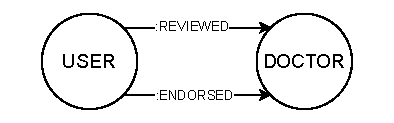
\includegraphics[scale=1.7]{./resources/neo4j.pdf}
    \caption{GraphDB structure for HealthHub}
    \label{fig:neo4j-structure}
\end{figure}

Our graph database (Figure~\ref{fig:neo4j-structure}) models two main entities:

\begin{itemize}
  \item \texttt{User}
  \item \texttt{Doctor}
\end{itemize}

Each node retains the MongoDB identifier to maintain consistency across databases. Neo4j is used selectively, focusing on relationship patterns and core attributes needed for traversal and inference, while full entity details remain in MongoDB.

The graph database plays a central role in modeling the social structure of the platform and is exploited in two main ways:
\begin{enumerate}
  \item As a \textbf{recommendation engine}, suggesting doctors to users based on graph proximity and shared review patterns.
  \item As a \textbf{search optimization layer}, improving query efficiency by leveraging graph traversal capabilities.
\end{enumerate}

Due to the lack of geographic data, we approximate location by leveraging graph proximity, under the assumption that users typically visit doctors near them. This enables us to infer locality-aware clusters and improve personalization without explicit spatial attributes.

\subsection{Node Types}

Neo4j stores only a minimal subset of each entity:
\begin{itemize}
  \item \textbf{User} nodes: \texttt{name}, \texttt{\_id}.
  \item \textbf{Doctor} nodes: \texttt{name}, \texttt{specializations}, \texttt{\_id}.
\end{itemize}

This lean representation minimizes redundancy while supporting all graph-based operations.

\subsection{Relationships}

We define two types of directed edges:
\begin{itemize}
  \item \textbf{:REVIEWED} — if user \texttt{U} has reviewed doctor \texttt{D}, then a \texttt{:REVIEWED} relationship is created from $U$ to $D$:  
  \[
    \texttt{U} \xrightarrow{\texttt{:REVIEWED}} \texttt{D}
  \]

  \item \textbf{:ENDORSED} — if user \texttt{U} endorsed doctor \texttt{D} (e.g., marked them as a favorite or recommended), we store this with a \texttt{:ENDORSED} relationship:  
  \[
    \texttt{U} \xrightarrow{\texttt{:ENDORSED}} \texttt{D}
  \]
\end{itemize}

These relations enable pattern discovery and inference. Spatial behavior is indirectly modeled through interaction patterns, which often reflect geographic closeness.

\section{Distributed Database Design}

\subsection{Replica Set Deployment}

\begin{figure}[t]
    \centering
    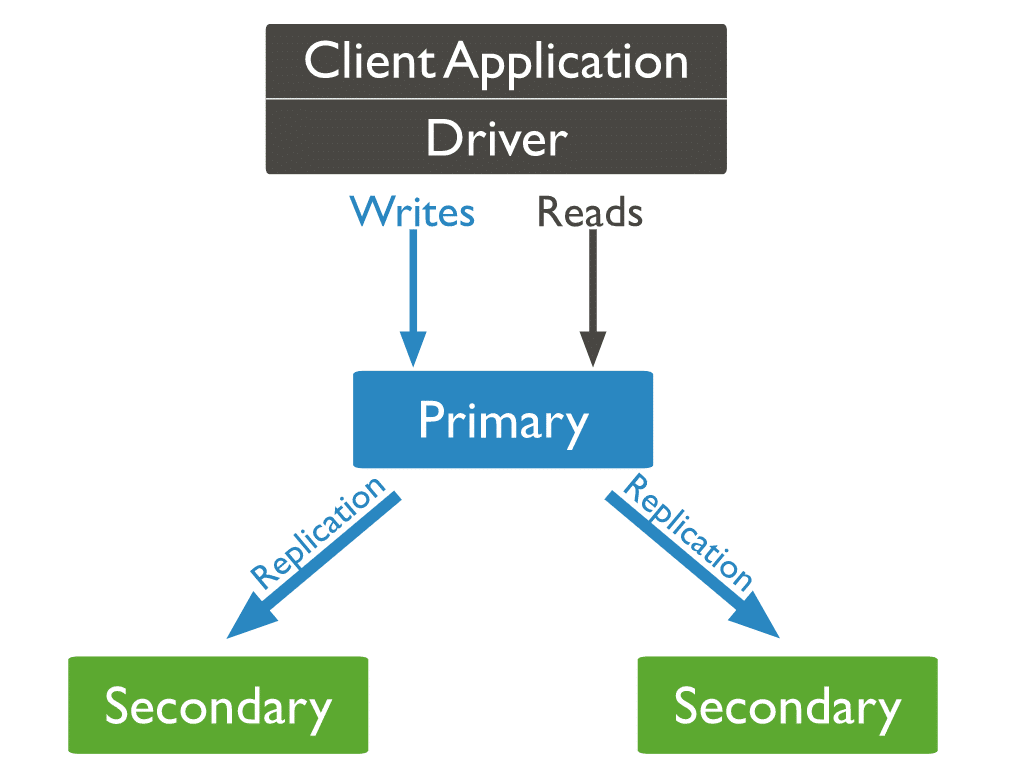
\includegraphics[scale=0.2]{./resources/mongo_replica.png}
    \caption{MongoDB Replica Set Structure}
    \label{fig:mongo-replica}
\end{figure}

We were given access to a cluster composed of three nodes. On each node, we deployed a MongoDB instance as part of a replica set. Neo4j was deployed in standalone mode, as replication requires the Enterprise edition, which was not available.

In the MongoDB replica set, only the \textbf{primary node} handles write operations. Each write is logged in the primary’s \emph{oplog} (operation log), which is then replicated to the \textbf{secondary nodes}. These secondaries apply the operations in the same order to maintain a consistent dataset. While all members of the replica set can serve read operations, by default, the application is configured to read from the primary node to preserve strong consistency.

\paragraph{Consistency Level}

Consistency across replicas is determined by the acknowledgment settings used during read and write operations. Our system adopts a hybrid consistency strategy:

\begin{itemize}
  \item The \texttt{write concern} is set to \texttt{w:1}, meaning that a write is acknowledged as soon as it has been applied by the primary node.
  \item The \texttt{read concern} is generally set to \texttt{local} (\texttt{r:1}), allowing reads from the local state of a node, which may not reflect the latest writes.
  \item However, for critical data such as a doctor's availability schedule, we explicitly enforce \texttt{readConcernLevel=majority} to ensure that only the most up-to-date and replicated information is retrieved.
\end{itemize}

This approach enables us to maintain \textbf{eventual consistency} where acceptable — improving performance and reducing latency — while enforcing \textbf{strong consistency} only in the specific cases that require it. It provides a good balance between responsiveness and data reliability, especially in a system that emphasizes availability and user experience.

\paragraph{CAP Theorem Considerations}

Our architecture emphasizes the \textbf{Availability (A)} and \textbf{Partition Tolerance (P)} aspects of the CAP theorem. The system is designed to:
\begin{itemize}
  \item Remain accessible and operational even during node failures or network partitions.
  \item Avoid sacrificing user responsiveness, ensuring that essential features—like searching doctors or leaving endorsements—remain available under most failure scenarios.
\end{itemize}

\subsection{Sharding (Design Perspective)}

Sharding has not been implemented in the current system but was considered as a viable strategy to scale the document database in case of high demand.

\paragraph{Horizontal Partitioning Strategy}

Sharding would be employed solely on the MongoDB side, as distributing a graph database like Neo4j across nodes introduces significant traversal overhead that defeats its performance benefits.

We proposed the following sharding design:

\begin{itemize}
  \item \textbf{Doctors Collection}:
    \begin{itemize}
      \item \textbf{Shard Key}: \texttt{address.province}
      \item \textbf{Sharding Mechanism}: hash-based
    \end{itemize}
    This approach would evenly distribute documents geographically, avoiding load concentration in specific provinces.

  \item \textbf{Appointments Collection}:
    \begin{itemize}
      \item \textbf{Shard Key}: \texttt{appointmentDateTime}
      \item \textbf{Sharding Mechanism}: range-based
    \end{itemize}
    Optimized for time-range queries, this configuration would support efficient access to recent or upcoming appointments.
\end{itemize}

These design options would ensure balanced workloads and scalable query processing if user and appointment volumes significantly increase in the future.

\subsection{Handling Inter-database Consistency}

Given that we use both a document-oriented database (MongoDB) and a graph database (Neo4j), some redundancy exists across the systems. Certain information—such as user endorsements—must be stored and updated in both databases.

To ensure consistency, we follow a two-phase update pattern:
\begin{itemize}
  \item A write operation is first performed on MongoDB.
  \item Only if the MongoDB operation is successful, the corresponding write on Neo4j is triggered.
  \item If the Neo4j update fails, a rollback is initiated to restore the system to a consistent state.
\end{itemize}

This logic is managed using Spring’s \texttt{@Transactional} annotation, ensuring atomicity across operations. Additionally, asynchronous execution is enabled via \texttt{@Async}, allowing long-running updates to Neo4j to execute in separate threads, enhancing system availability.

\begin{figure}[!ht]
    \centering
    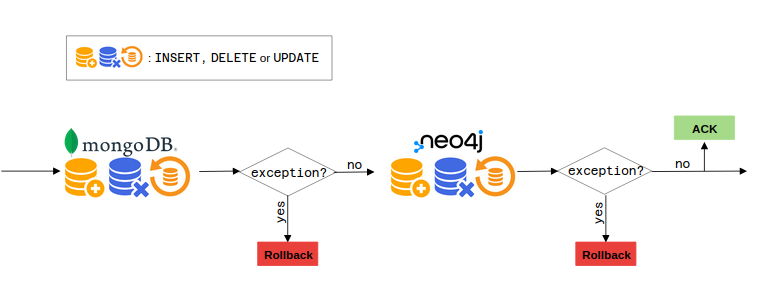
\includegraphics[scale=0.5]{./resources/rollback.png}
    \caption{Handling consistency between MongoDB and Neo4j}
    \label{fig:mongo-neo4j-sync}
\end{figure}

\paragraph{Eventual Consistency and Responsiveness}

The system is designed to tolerate brief inconsistencies between MongoDB and Neo4j. This decision improves performance and responsiveness—key aspects for a user-focused social system. Consistency is restored asynchronously and transparently, without impacting the user experience.

\chapter{Implementation}
\section{Front-End}
The front-end of our application has been developed as a traditional web-based interface, utilizing a combination of \textbf{JavaScript}, \textbf{HTML} and \textbf{CSS}. This technology stack enables the creation of a responsive and interactive user interface that can be accessed from any modern web browser without the need for additional installations. The application communicates asynchronously with the back-end server through \textbf{AJAX} (Asynchronous JavaScript and XML) requests, allowing data to be fetched and updated dynamically without requiring full page reloads. This results in a smoother user experience and improved performance, particularly when handling operations such as appointment booking, profile managementand real-time data visualization. The separation of concerns between presentation and logic also enhances the maintainability and scalability of the application.

\section{Front-End Structure}
The \textbf{resources} directory encapsulates the front-end assets and configuration files essential to the operation and presentation of the web application. Its hierarchical organization reflects a separation of concerns, promoting maintainability and modular development.

Static resources such as CSS and JavaScript files reside in the \textbf{static} folder, structured into subdirectories for stylesheets (\textbf{css/}), scripts (\textbf{js/}) and error pages (\texttt{error/}). These support the visual and interactive components of the application.

Dynamic \textbf{HTML} views based on \textbf{Thymeleaf} are located in the \textbf{templates} folder, with dedicated files for both doctors and users. A \textbf{fragments} subfolder contains reusable layout components (e.g., headers, footers, sidebars) to ensure consistency and reusability. Application-level configuration is managed through \texttt{application.properties}.

\subsection{Static}
The \textbf{static} directory collects all static web assets that are delivered to the client without server-side processing. These assets are organized into three primary subfolders: \texttt{css/}, \texttt{js/}, and \texttt{error/}, each serving a distinct role in the client-side rendering process.

The \textbf{css} folder contains a series of modular stylesheets dedicated to specific views or components. These include both general-purpose files (e.g. \texttt{base.css}, \texttt{main.css}, \texttt{form.css}) and context-specific styles (e.g. \texttt{doctor-dashboard.css}, \texttt{user-profile.css}), which define the visual identity and layout of user and doctor interfaces.

The \textbf{js} folder hosts JavaScript files that manage client-side interactions and dynamic behavior. Each script is associated with a specific view or functionality—for instance, \texttt{login.js} handles authentication interactions, while \texttt{slot-calendar.js} governs dynamic calendar updates for appointment scheduling.

The \textbf{error} folder includes static HTML pages for standard HTTP error responses (400, 404, 500), ensuring that users receive consistent and informative feedback in case of failure scenarios.

This structure promotes modularity and clarity, allowing for straightforward maintenance and scalability of front-end assets.

\subsection{Templates}
The \texttt{templates} directory constitutes a fundamental component within the presentation layer of the web application, as it houses the markup resources responsible for rendering the user interface. This directory is hierarchically organized into subfolders, each reflecting a specific functional domain or interaction paradigm with which the user engages. The HTML documents contained therein are primarily structured using Thymeleaf, a server-side template engine designed for Java-based web environments.

Thymeleaf facilitates the synthesis of dynamic HTML views on the server side, enabling the embedding of context-sensitive data—such as session attributes, query outputsand user-submitted form content—directly into the markup prior to delivery to the client. This server-side rendering paradigm promotes a high degree of interactivity and allows for the generation of customized and context-aware web pages, thereby improving the overall responsiveness and user-centricity of the application interface.

\section{Back-End}
The back-end is implemented using \textbf{Java} due to its robustness, platform independenceand strong ecosystem. Java offers a well-established set of libraries and frameworks that support rapid development of secure, scalableand maintainable web applications. Its object-oriented nature encourages clean architecture and modular design, which are essential for complex systems like healthcare platforms. Additionally, Java's widespread use in enterprise environments ensures long-term support and community-driven innovation, making it a reliable choice for production-grade applications.

\subsection{Spring Boot}
As the core of our application, we adopted the \textbf{Spring Boot} framework, which has significantly streamlined both the development and deployment processes. One of the primary advantages of Spring Boot lies in its built-in support for an embedded \textbf{Tomcat} server, allowing the creation of a fully functional web application without requiring external configuration. This design choice has enhanced our ability to construct responsive and maintainable RESTful APIs. 

In addition, to support our data management needs, we integrated \textbf{Spring Data Neo4j} and \textbf{Spring Data MongoDB}. The former facilitates interaction with the \textbf{Neo4j graph database} through a consistent repository-based abstraction, ideal for managing highly interconnected medical data such as relationships between doctors and patients. The latter offers seamless integration with \textbf{MongoDB}, \textbf{a document-oriented NoSQL database}, while preserving the flexibility and idiomatic programming style of the broader Spring ecosystem. Collectively, these technologies have provided a robust, scalable and modular architecture well-suited to the requirements of our application. 

\section{Back-End Structure}
The application follows the layered architecture presented during lectures, organizing the codebase into clearly defined packages to promote modularity and separation of concerns. 

\subsection{\texttt{package it.unipi.healthhub.config}}
The \textbf{Config} package usually contains configuration classes. In our case, we have only one class. 

The \texttt{FilterConfig} class defines the registration of custom servlet filters used to manage access control within the application. Annotated with \texttt{@Configuration}, it registers filters via \texttt{FilterRegistrationBean}, associating each filter with specific URL patterns. 

In detail:
\begin{itemize}
	\item \texttt{DoctorDashboardAuthFilter}: restricts access to \texttt{/doctor/dashboard/*};
	\item \texttt{PatientDashboardFilter}: applied to \texttt{/user/*};
	\item \texttt{PatientApiFilter}: secures \texttt{/api/user/*};
	\item \texttt{DoctorApiFilter}: secures \texttt{/api/doctor/*};
	\item \texttt{LoginFilter}: manages access to the login page at \texttt{/login}.
\end{itemize}

\subsection{\texttt{package it.unipi.healthhub.controller}}
The \texttt{Controller} package manages API endpoint mappings and web page controllers for the core sections of the application, including the homepage, login, registrationand doctor dashboard. All classes in this package follow the Spring MVC (Model-View-Controller) framework, ensuring a clean separation of concerns between business logic, HTTP request handlingand view rendering.

More spefically:
\begin{itemize}
	\item The \texttt{AuthController} handles authentication and registration processes for both patients (users) and doctors. Its responsibilities include rendering login, registrationand password recovery views; managing user sessions; creating new user accounts; and processing password reset requests. Utility classes such as \texttt{ControllerUtil} and \texttt{HashUtil} are employed to promote modularity and code reuse.
	\item The \texttt{DoctorController} manages requests related to viewing a doctor’s public profile. It retrieves the corresponding data via the \texttt{DoctorService} and injects it into the model for view rendering.
	\item The \texttt{DoctorDashboardController} supports navigation within the doctor's dashboard by mapping each HTTP GET request to a specific section such as appointments, profile, reviews, templatesand weekly schedule. It retrieves the authenticated doctor's data from the session and delegates business logic to the \texttt{DoctorService}.
	\item The \texttt{HomeController} handles requests to the root endpoints (\texttt{/}, \texttt{/index}) and to the \texttt{/search} page. Each method ensures that session-specific data is consistently added to the model using \texttt{ControllerUtil} before returning the appropriate view.
	\item The \texttt{UserController} manages authenticated user interactions through endpoints under \texttt{/user}, including profile viewing, appointmentsand favorite doctors. It uses \texttt{ControllerUtil} to populate the model with session-based data. The class adopts a session-aware MVC design aimed at personalized user interaction.
\end{itemize}

\subsection{\texttt{package it.unipi.healthhub.controller.api}}
The \texttt{it.unipi.healthhub.controller.api} package defines a set of RESTful controllers that expose the application's core services via HTTP endpoints. These controllers are designed to return data (typically in JSON format) allowing asynchronous communication with frontend components and third-party systems.

Serving as the API layer of the system architecture, this package supports decoupled access to key resources such as users, doctors, appointmentsand reviews. It complements the standard MVC controllers by enabling machine-oriented interactions, in alignment with modern web application practices.

\subsubsection{DoctorAPI}
The \texttt{DoctorAPI} class defines a RESTful web interface to manage and interact with doctor-related resources within the \textit{HealthHub} system. It is annotated with \texttt{@RestController} and is mapped to the base path \texttt{/api/doctors}. Below is a summary of the main endpoints:

\begin{itemize}
	\item \texttt{GET /api/doctors} \\
	Returns a list of all registered doctors.
	
	\item \texttt{GET /api/doctors/\{id\}} \\
	Retrieves a specific doctor by their unique identifier.
	
	\item \texttt{POST /api/doctors} \\
	Creates a new doctor resource.
	
	\item \texttt{PUT /api/doctors/\{id\}} \\
	Updates an existing doctor identified by \texttt{id}.
	
	\item \texttt{DELETE /api/doctors/\{id\}} \\
	Deletes the doctor with the specified \texttt{id}.
	
	\item \texttt{GET /api/doctors/\{doctorId\}/services} \\
	Retrieves the list of services offered by the specified doctor.
	
	\item \texttt{GET /api/doctors/\{doctorId\}/appointments} \\
	Returns the list of appointments associated with a doctor.
	
	\item \texttt{POST /api/doctors/\{doctorId\}/appointments} \\
	Books an appointment for the authenticated patient with the given doctor.
	
	\item \texttt{GET /api/doctors/\{doctorId\}/templates} \\
	Retrieves scheduling templates used by the doctor.
	
	\item \texttt{GET /api/doctors/\{doctorId\}/schedules/week?year=\dots\&week=\dots} \\
	Returns the weekly schedule (including prenotable slots) for a doctor, given the ISO week and year.
	
	\item \texttt{GET /api/doctors/\{doctorId\}/endorsements} \\
	Retrieves the total number of endorsements for a doctor and whether the current user has endorsed them.
	
	\item \texttt{POST /api/doctors/\{doctorId\}/endorse} \\
	Allows a logged-in patient to endorse a doctor.
	
	\item \texttt{POST /api/doctors/\{doctorId\}/unendorse} \\
	Removes an existing endorsement made by the patient.
	
	\item \texttt{GET /api/doctors/\{doctorId\}/reviews} \\
	Returns all patient reviews for the specified doctor.
	
	\item \texttt{POST /api/doctors/\{doctorId\}/reviews} \\
	Submits a review for a doctor, provided the patient has had an appointment with them.
	
	\item \texttt{GET /api/doctors/\{doctorId\}/reviews/week/count} \\
	Returns the number of reviews a doctor received during the current ISO week.
\end{itemize}

\subsubsection{PrivateDoctorAPI}
The \texttt{PrivateDoctorAPI} class implements a secure REST interface for authenticated doctors to manage their personal data, appointmentsand analytic insights. Annotated with \texttt{@RestController} and mapped to \texttt{/api/doctor}, it delegates domain logic to \texttt{AppointmentService} and \texttt{DoctorService}, enforcing session‐based access control. Below is a summary of the main endpoints:

\begin{itemize}
	\item \texttt{GET /api/doctor/appointments} \\
	retrieves today's appointments (or for a given date).
	\item \texttt{DELETE /api/doctor/appointments/\{id\}} \\
	deletes an appointment.
	\item \texttt{PUT /api/doctor/address} \\
	updates the doctor's address.
	\item \texttt{PUT /api/doctor/info} \\
	updates the doctor's profile info.
	\item \texttt{POST /api/doctor/phone} \\
	adds a phone number.
	\item \texttt{DELETE /api/doctor/phone/\{index\}} \\
	removes a phone number by a doctor.
	\item \texttt{POST /api/doctor/specialization} \\
	adds a specialization.
	\item \texttt{DELETE /api/doctor/specialization/\{index\}} \\
	removes a specialization.
	\item \texttt{POST /api/doctor/service} \\
	adds a medical service.
	\item \texttt{GET /api/doctor/service} \\
	retrieves all offered services.
	\item \texttt{PUT /api/doctor/service} \\
	updates a medical service.
	\item \texttt{DELETE /api/doctor/service/\{id\}} \\
	deletes a medical service.
	\item \texttt{POST /api/doctor/template} \\
	creates a new availability template.
	\item \texttt{GET /api/doctor/template} \\
	retrieves all availability templates.
	\item \texttt{PUT /api/doctor/template} \\
	updates a template. 
	\item \texttt{DELETE /api/doctor/template/\{id\}} \\
	deletes a template.
	\item \texttt{PUT /api/doctor/template/default} \\
	sets the default availability template.
	\item \texttt{POST /api/doctor/schedule} \\
	creates a weekly schedule.
	\item \texttt{GET /api/doctor/schedule} \\
	retrieves the weekly schedule.
	\item \texttt{PUT /api/doctor/schedule} \\
	updates the weekly schedule.
	\item \texttt{DELETE /api/doctor/schedule} \\
	deletes the weekly schedule.
	\item \texttt{GET /api/doctor/reviews} \\
	retrieves all received reviews.
	\item \texttt{DELETE /api/doctor/review/\{id\}} \\
	deletes a review.
	\item \texttt{PUT /api/doctor/password} \\
	changes the password.
	\item \texttt{GET /api/doctor/stats/visits}\\
	gets number of visits (optionally weekly).
	\item \texttt{GET /api/doctor/stats/earnings}\\
	gets annual earnings.
	\item \texttt{GET /api/doctor/stats/patients} \\
	gets number of new patients per month.
\end{itemize}

\subsubsection{UserAPI}
The \texttt{UserAPI} controller is a RESTful web service component. It provides endpoints for managing user entities within the HealthHub application, leveraging the \texttt{UserService} to perform CRUD (Create, Read, Update, Delete) operations on patients stored in a MongoDB database. The controller follows standard REST conventions, utilizing HTTP verbs to represent actions on resources. 

\begin{itemize}
	\item \texttt{GET /api/users} \\
	Retrieves a list of all users registered in the system.
	
	\item \texttt{GET /api/users/\{id\}} \\
	Fetches a specific user by their unique identifier. Returns HTTP 200 with the user data if found, otherwise HTTP 404.
	
	\item \texttt{POST /api/users} \\
	Creates a new user entity based on the data provided in the request body. Returns the created user.
	
	\item \texttt{PUT /api/users/\{id\}} \\
	Updates an existing user identified by the given ID with new data provided in the request body. Returns HTTP 200 with the updated user if the operation is successful; returns HTTP 404 if the user does not exist.
	
	\item \texttt{DELETE /api/users/\{id\}} \\
	Deletes the user identified by the specified ID. Returns HTTP 204 No Content regardless of whether the user existed, indicating that the request has been processed.
\end{itemize}

\subsubsection{PrivateUserAPI}
The \texttt{PrivateUserAPI} controller is a RESTful web service implemented using the Spring framework in Java, designed to provide secured endpoints for user-specific operations within the HealthHub system. It leverages HTTP sessions to identify the authenticated user (typically a patient) and delegates business logic to the \texttt{UserService}. The controller exposes various endpoints to manage user details, contacts, appointments, doctor recommendationsand password changes, emphasizing privacy and personalization.

\begin{itemize}
	\item \texttt{GET /api/user/details} \\
	Retrieves detailed personal information of the currently authenticated user by extracting the patient ID from the HTTP session. Returns user details or an error message in case of failure.
	
	\item \texttt{PUT /api/user/details} \\
	Updates the personal details of the authenticated user. The new data is supplied in the request body as a \texttt{UserDetailsDTO} object.
	
	\item \texttt{GET /api/user/details/view?id=\{id\}} \\
	Retrieves contact information and demographic data for a user specified by the \texttt{id} query parameter. Additionally, if a doctor is logged in, it returns the number of visits that doctor has conducted with the user.
	
	\item \texttt{GET /api/user/contacts} \\
	Fetches the contact information related to the authenticated user.
	
	\item \texttt{PUT /api/user/contacts} \\
	Updates the contact information of the authenticated user using data provided in the request body as a \texttt{PatientContactsDTO}.
	
	\item \texttt{GET /api/user/appointments/upcoming} \\
	Retrieves a list of upcoming appointments for the authenticated user.
	
	\item \texttt{GET /api/user/appointments/past} \\
	Retrieves a list of past appointments for the authenticated user.
	
	\item \texttt{DELETE /api/user/appointments/\{appointmentId\}} \\
	Cancels the appointment identified by \texttt{appointmentId}. Returns HTTP 200 on success or HTTP 400 if the appointment does not exist.
	
	\item \texttt{GET /api/user/recommendations?limit=\{limit\}} \\
	Returns a list of recommended doctors for the authenticated user, with an optional parameter \texttt{limit} to specify the maximum number of results (default is 3).
	
	\item \texttt{GET /api/user/doctors/reviewed} \\
	Returns a list of doctors that the authenticated user has reviewed.
	
	\item \texttt{GET /api/user/doctors/endorsed} \\
	Returns a list of doctors endorsed by the authenticated user.
	
	\item \texttt{PUT /api/user/password} \\
	Allows the authenticated user to change their password. The current and new passwords are supplied in the request body as a \texttt{PasswordChangeDTO} and are hashed before validation and update.
\end{itemize}

\subsubsection{SearchAPI}
The \texttt{SearchAPI} controller is a RESTful component, responsible for executing search queries specifically targeted at medical doctors within the HealthHub system. This controller integrates data from two distinct data sources: a MongoDB database and a Neo4j graph database. The rationale behind this dual-source approach is to combine traditional document-oriented search results with personalized recommendations derived from graph-based relationships. 

The primary endpoint exposed by this controller is: \texttt{GET /api/search/doctors}.  
This endpoint accepts a mandatory \texttt{query} parameter, representing the search string to be matched against doctor records. Additionally, it accesses the HTTP session to retrieve the identifier of the currently authenticated patient (if available), enabling personalized search refinement. 

Upon receiving a valid query, the controller queries the MongoDB database via \texttt{DoctorService}, returning results as \texttt{DoctorMongoProjection} objects that represent doctor records optimized for search display. If the user is unauthenticated or the patient identifier is absent, the controller returns the top ten doctors from the MongoDB results, sorted by relevance.

For authenticated users, the controller enriches the search outcomes by querying the Neo4j graph database to retrieve personalized recommendations. These recommendations are returned as \texttt{DoctorNeo4jProjection} objects, each associated with a relevance score reflecting the strength of the doctor-patient relationship, such as prior interactions or endorsements. In the absence of Neo4j results, the system falls back to the top MongoDB results.

The integration of results from both sources is achieved by mapping doctor identifiers to Neo4j scores, then augmenting each MongoDB doctor's score accordingly. Doctors without Neo4j matches receive a default negative score to denote lack of personalized relevance. The aggregated list is sorted in descending order by combined scoreand the top ten entries are converted into \texttt{DoctorDTO} objects for API response consistency.

Two private helper methods, \texttt{toDto} and \texttt{toTop10Dto}, support this process by converting raw entities to DTOs and by sorting and limiting the result set. This design ensures that search responses maintain a uniform format, whether or not personalization is applied. Overall, the \texttt{SearchAPI} exemplifies a hybrid search strategy that effectively merges traditional document-based retrieval with graph-driven personalization, leveraging session data to optimize relevance and incorporating fallback mechanisms to ensure robust performance for both authenticated and anonymous users.

\subsection{\texttt{package it.unipi.healthhub.dto}}
The Data Transfer Objects (DTO) directory encapsulates a set of plain Java objects that serve as data carriers between different layers of the HealthHub application, primarily facilitating communication between the service and presentation tiers. These DTO classes are designed to aggregate and structure data relevant to specific business operations or user interactions, decoupling the internal domain model from external API contracts.

\subsection{\texttt{package it.unipi.healthhub.exception}}
The \texttt{it.unipi.healthhub.exception} package defines a set of custom unchecked exceptions, each extending \texttt{RuntimeException}, to represent specific error conditions encountered in the HealthHub application’s domain logic. By encapsulating distinct failure scenarios—such as missing resources or duplicate entries—these exceptions facilitate clear error propagation and centralized handling in higher layers (e.g., controllers or global exception handlers). Moreover, they improve code readability by replacing generic error signals with semantically meaningful types.

\begin{itemize}
	\item \texttt{DoctorNotFoundException}:  
	Thrown when an operation attempts to retrieve or manipulate a doctor entity that does not exist in the system. Constructors allow for default or custom error messagesand for nesting an underlying cause;
	
	\item \texttt{ScheduleAlreadyExistsException}:  
	Raised to indicate an attempt to create a schedule for a doctor in a week for which a schedule is already defined. This prevents conflicting availability entries. As with other exceptions, it supports message customization and cause propagation;
	
	\item \texttt{UserAlreadyExistsException}:  
	Used when a registration or user-creation process detects that a user with the same unique identifier (e.g., email or fiscal code) is already present in the database. This exception enforces uniqueness constraints at the application layer;
	
	\item \texttt{UserNotFoundException}:  
	Thrown when a requested user resource cannot be found, for instance during authentication, profile retrieval, or update operations. Its constructors mirror those of the other exception types, enabling flexible error reporting.
\end{itemize}

\subsection{\texttt{package it.unipi.healthhub.filter}}
The \texttt{it.unipi.healthhub.filter} package provides servlet filters that centralize authentication and authorization logic for both API and web endpoints. These filters intercept incoming HTTP requests, verify session validity and user rolesand either allow processing to continue, redirect to the login page, or return appropriate HTTP error codes upon access violations.

\begin{itemize}
	\item \textbf{DoctorApiFilter}:
	Ensures that requests to \texttt{/api/doctor/*} originate from an authenticated doctor. If no session exists or the session attribute \texttt{role} is not \texttt{"doctor"}, the filter responds with HTTP 403 Forbidden;
	
	\item \textbf{DoctorDashboardAuthFilter}:
	Protects doctor dashboard pages under \texttt{/doctor/dashboard/*}. It verifies the presence of a valid session with \texttt{role = "doctor"}. If validation fails, the user is redirected to the login page;
	
	\item \textbf{LoginFilter}: 
	Prevents authenticated users from re‐accessing the login page. For existing sessions, GET requests to the login URL are redirected to \texttt{/index} (the home page), while POST attempts are rejected with HTTP 403 Forbidden;
	
	\item \textbf{PatientApiFilter}:
	Applies to \texttt{/api/user/*}, allowing read‐only GET requests for all users but restricting state‐changing methods (POST, PUT, DELETE) exclusively to authenticated patients (session attribute \texttt{role = "patient"}). Unauthorized modification attempts yield HTTP 403 Forbidden;
	
	\item \textbf{PatientDashboardFilter}:
	Secures patient dashboard views under \texttt{/user/*}. It checks for an active session with \texttt{role = "patient"} and redirects unauthenticated or improperly privileged users to the login page.
\end{itemize}

\subsection{\texttt{package it.unipi.healthhub.model}}
The \textbf{Model} package defines the entity classes corresponding to the database schema.

The \texttt{it.unipi.healthhub.model.mongo} package contains the core domain entities persisted in MongoDB. These classes represent the primary data models for the application and include:

\begin{itemize}
	\item \textbf{Address.java}: encapsulates patient or doctor address fields (street, city, province, postal code and country);
	\item \textbf{Appointment.java}: models appointment records, linking patients and doctors with date, time and status.;
	\item \textbf{CalendarTemplate.java}: defines named availability templates composed of slot collections;
	\item \textbf{Doctor.java}: represents doctor profiles, including personal details, specializations and business rules;
	\item \textbf{PrenotableSlot.java}: denotes individual time slots available for booking;
	\item \textbf{Review.java}: captures patient‑submitted reviews;
	\item \textbf{Schedule.java}: organizes weekly schedules as mappings from days to prenotable slots;
	\item \textbf{Service.java}: specifies medical services offered by a doctor, including descriptions and pricing;
	\item \textbf{Slot.java}: a simple time interval used within templates and schedules;
	\item \textbf{User.java}: models patient accounts with personal information and secure credentials.
\end{itemize}

In addition, the \texttt{it.unipi.healthhub.model.neo4j} subpackage defines lightweight DAO classes (\textbf{DoctorDAO.java}, \textbf{UserDAO.java}) used exclusively for graph queries. Since all entity attributes required by the application are already captured in the MongoDB models and relationships are managed via Neo4j projections, the MongoDB classes serve as the definitive domain models.

Their structural design has already been detailed in the Design chapter’s UML class diagram section.

\subsection{\texttt{package it.unipi.healthhub.model.mongo}}
\subsubsection{User}
\begin{lstlisting}[language=java]
@Document(collection = "users")
public class User {
	@Id
	protected String id;
	
	protected String username;
	
	protected String name;
	protected String password;
	protected String fiscalCode;
	protected LocalDate dob;
	protected String gender;
	private String personalNumber;
	protected String email;
	
	public String getId() {
		return id;
	}
	public void setId(String id) { this.id = id; }
	public String getName() {
		return name;
	}
	public void setName(String name) {
		this.name = name;
	}
	public String getUsername() {
		return username;
	}
	public void setUsername(String username) {
		this.username = username;
	}
	
	public String getFiscalCode(){ return fiscalCode; }
	public void setFiscalCode(String fiscalCode){ this.fiscalCode = fiscalCode; }
	
	public String getGender() {
		return gender;
	}
	public void setGender(String gender) {
		this.gender = gender;
	}
	
	public String getEmail() {
		return email;
	}
	public void setEmail(String email) {
		this.email = email;
	}
	
	public String getPassword() {
		return password;
	}
	public void setPassword(String password) {
		this.password = password;
	}
	
	public void setDob(LocalDate dob) {
		this.dob = dob;
	}
	public LocalDate getDob() {
		return dob;
	}
	
	public String getPersonalNumber() {
		return personalNumber;
	}
	
	public void setPersonalNumber(String personalNumber) {
		this.personalNumber = personalNumber;
	}
	
	public String toString() {
		return "User{" +
			", username='" + username + '\'' +
			", password='" + password + '\'' +
			", dob=" + dob + "}";
	}
}
\end{lstlisting}

\subsubsection{}
\begin{lstlisting}[language=java]
	@Document(collection = "doctors")
	public class Doctor extends User {
		protected String orderRegistrationNumber;
		private List<Service> services;
		private int endorsementCount;
		private int reviewCount;
		private List<Review> reviews;
		private List<Schedule> schedules;
		private List<String> calendarTemplates;
		private List<String> specializations;
		private List<String> phoneNumbers;
		private Address address;
		
		public Doctor() {
			super();
			services = new ArrayList<>();
			reviews = new ArrayList<>();
			schedules = new ArrayList<>();
			calendarTemplates = new ArrayList<>();
			specializations = new ArrayList<>();
			phoneNumbers = new ArrayList<>();
		}
		
		public String getOrderRegistrationNumber() { return orderRegistrationNumber; }
		public void setOrderRegistrationNumber(String orderRegistrationNumber) { this.orderRegistrationNumber = orderRegistrationNumber; }
		
		public List<Service> getServices() {
			return services;
		}
		public void setServices(List<Service> services) {
			this.services = services;
		}
		
		public int getEndorsementCount() {
			return endorsementCount;
		}
		public void setEndorsementCount(int endorsementCount) {
			this.endorsementCount = endorsementCount;
		}
		
		public int getReviewCount() {
			return reviewCount;
		}
		public void setReviewCount(int reviewCount) { this.reviewCount = reviewCount; }
		
		public List<Review> getReviews() {
			return reviews;
		}
		public void setReviews(List<Review> reviews) {
			this.reviews = reviews;
		}
		
		public List<Schedule> getSchedules() {
			return schedules;
		}
		public void setSchedules(List<Schedule> schedules) {
			this.schedules = schedules;
		}
		
		public List<String> getCalendarTemplates() {
			return calendarTemplates;
		}
		public void setCalendarTemplates(List<String> calendarTemplates) {
			this.calendarTemplates = calendarTemplates;
		}
		
		public List<String> getSpecializations() {
			return specializations;
		}
		public void setSpecializations(List<String> specializations) {
			this.specializations = specializations;
		}
		
		public List<String> getPhoneNumbers() {
			return phoneNumbers;
		}
		public void setPhoneNumbers(List<String> phoneNumbers) {
			this.phoneNumbers = phoneNumbers;
		}
		
		public Address getAddress() {
			return address;
		}
		public void setAddress(Address address) {
			this.address = address;
		}
		
		public String getId(){
			return super.getId();
		}
		
		public String toString() {
			return "User{" +
				", username='" + getUsername() + '\'' +
				", password='" + getPassword() + '\'' +
				", dob=" + dob + "}";
		}
	}
\end{lstlisting}

\subsubsection{Appointment}
\begin{lstlisting}[language=java]
@Document(collection = "appointments")
public class Appointment {
	@Id
	private String id;
	private LocalDateTime date;
	private DoctorInfo doctor;
	private PatientInfo patient;
	private String visitType;
	private String patientNotes;
	private double price;
	
	// Constructors
	public Appointment() {}
	
	public Appointment(String id, LocalDateTime appointmentDateTime, DoctorInfo doctorInfo, PatientInfo patientInfo, String visitType, String patientNotes) {
		this.id = id;
		this.date = appointmentDateTime;
		this.doctor = doctorInfo;
		this.patient = patientInfo;
		this.visitType = visitType;
		this.patientNotes = patientNotes;
	}
	
	// Getters and Setters
	public String getId() {
		return id;
	}
	
	public void setId(String id) {
		this.id = id;
	}
	
	public LocalDateTime getDate() {
		return date;
	}
	
	public void setDate(LocalDateTime date) {
		this.date = date;
	}
	
	public DoctorInfo getDoctor() {
		return doctor;
	}
	
	public void setDoctor(DoctorInfo doctor) {
		this.doctor = doctor;
	}
	
	public PatientInfo getPatient() {
		return patient;
	}
	
	public void setPatient(PatientInfo patient) {
		this.patient = patient;
	}
	
	public String getVisitType() {
		return visitType;
	}
	
	public void setVisitType(String visitType) {
		this.visitType = visitType;
	}
	
	public String getPatientNotes() {
		return patientNotes;
	}
	
	public void setPatientNotes(String patientNotes) {
		this.patientNotes = patientNotes;
	}
	
	public void setPrice(Double price) {
		this.price = price;
	}
	
	public double getPrice() {
		return price;
	}
	
	// Inner class DoctorInfo
	public static class DoctorInfo {
		private String id;
		private String name;
		private Address address;
		private String email;
		
		public DoctorInfo() {}
		
		public DoctorInfo(String doctorId, String doctorName, Address address, String email) {
			this.id = doctorId;
			this.name = doctorName;
			this.address = address;
			this.email = email;
		}
		
		public String getId() {
			return id;
		}
		
		public void setId(String id) {
			this.id = id;
		}
		
		public String getName() {
			return name;
		}
		
		public void setName(String name) {
			this.name = name;
		}
		
		public Address getAddress() {
			return address;
		}
		
		public void setAddress(Address address) {
			this.address = address;
		}
		
		public String getEmail() {
			return email;
		}
		
		public void setEmail(String email) {
			this.email = email;
		}
	}
	
	// Inner class PatientInfo
	public static class PatientInfo {
		private String id;
		private String name;
		private String email;
		private String gender;
		
		public PatientInfo() {}
		
		public PatientInfo(String patientId, String patientName, String email, String gender) {
			this.id = patientId;
			this.name = patientName;
			this.email = email;
			this.gender = gender;
		}
		
		public String getId() {
			return id;
		}
		
		public void setId(String id) {
			this.id = id;
		}
		
		public String getName() {
			return name;
		}
		
		public void setName(String name) {
			this.name = name;
		}
		
		public String getEmail() {
			return email;
		}
		
		public void setEmail(String email) {
			this.email = email;
		}
		
		public String getGender() {
			return gender;
		}
		
		public void setGender(String gender) {
			this.gender = gender;
		}
	}
}
\end{lstlisting}

\subsubsection{Address}
\begin{lstlisting}[language=java]
public class Address {
	private String street;
	private String city;
	private String province;
	private String postalCode;
	private String country;
	
	// Constructor
	public Address(String street, String city, String province, String postalCode, String country){
		this.street = street;
		this.city = city;
		this.province = province;
		this.postalCode = postalCode;
		this.country = country;
	}
	
	// Getters and Setters
	public String getStreet() {
		return street;
	}
	
	public void setStreet(String street) {
		this.street = street;
	}
	
	public String getCity() {
		return city;
	}
	
	public void setCity(String city) {
		this.city = city;
	}
	
	public String getProvince() {
		return province;
	}
	
	public void setProvince(String province) {
		this.province = province;
	}
	
	public String getPostalCode() {
		return postalCode;
	}
	
	public void setPostalCode(String postalCode) {
		this.postalCode = postalCode;
	}
	
	public String getCountry() {
		return country;
	}
	
	public void setCountry(String country) {
		this.country = country;
	}
	
	public String toString() {
		return street + ", " + city + ", " + province + ", " + postalCode + ", " + country;
	}
	
	public String toShortString() {
		return street + ", " + city;
	}
}
\end{lstlisting}

\subsubsection{Calendar Template}
\begin{lstlisting}[language=java]
	@Document(collection = "templates")
	public class CalendarTemplate {
		@Id
		private String id;
		private String name;
		private Map<String, List<Slot>> slots;
		private boolean isDefault;
		
		// Constructor
		public CalendarTemplate() {}
		
		public CalendarTemplate(String id, String name, Map<String, List<Slot>> slots, boolean isDefault) {
			this.id = id;
			this.name = name;
			this.slots = slots;
			this.isDefault = isDefault;
		}
		
		// Getters and Setters
		public String getId() {
			return id;
		}
		
		public void setId(String id) {
			this.id = id;
		}
		
		public String getName() {
			return name;
		}
		
		public void setName(String name) {
			this.name = name;
		}
		
		public Map<String, List<Slot>> getSlots() {
			return slots;
		}
		
		public void setSlots(Map<String, List<Slot>> slots) {
			this.slots = slots;
		}
		
		public boolean isDefault(){
			return isDefault;
		}
		
		public void setDefault(boolean isDefault) {
			this.isDefault = isDefault;
		}
		
		public String toString() {
			return "CalendarTemplate{" +
				"id='" + id + '\'' +
				", name='" + name + '\'' +
				", slots=" + slots +
				", default=" + isDefault +
				'}';
		}
		
	}
\end{lstlisting}

\subsubsection{Prenotable Slot}
\begin{lstlisting}[language=java]
	public class PrenotableSlot extends Slot{
		private boolean taken;
		
		public PrenotableSlot() {
			super();
		}
		
		public PrenotableSlot(String start, String end, boolean taken) {
			super(start, end);
			this.taken = taken;
		}
		
		public boolean isTaken() {
			return taken;
		}
		
		public void setTaken(boolean taken) {
			this.taken = taken;
		}
	}
\end{lstlisting}

\subsubsection{Review}
\begin{lstlisting}[language=java]
	public class Review {
		public String name;
		public String text;
		public LocalDate date;
		public String patientId;
		
		public String getName() {
			return name;
		}
		public void setName(String name) {
			this.name = name;
		}
		
		public String getText() {
			return text;
		}
		public void setText(String text) {
			this.text = text;
		}
		
		public LocalDate getDate() {
			return date;
		}
		public void setDate(LocalDate date) {
			this.date = date;
		}
		
		public String getPatientId() {
			return patientId;
		}
		public void setPatientId(String patientId) {
			this.patientId = patientId;
		}
	}
\end{lstlisting}

\subsubsection{Schedule}
\begin{lstlisting}[language=java]
	public class Schedule {
		private LocalDate week;
		private Map<String, List<PrenotableSlot>> slots;
		
		// Getters and Setters
		public LocalDate getWeek() {
			return week;
		}
		
		public void setWeek(LocalDate week) {
			this.week = week;
		}
		
		public Map<String, List<PrenotableSlot>> getSlots() {
			return slots;
		}
		
		public void setSlots(Map<String, List<PrenotableSlot>> slots) {
			this.slots = slots;
		}
	}
\end{lstlisting}

\subsubsection{Service}
\begin{lstlisting}[language=java]
	public class Service {
		private String service;
		private double price;
		
		// Constructors
		public Service() {}
		public Service(String service, double price) {
			this.service = service;
			this.price = price;
		}
		
		// Getters and Setters
		public String getService() {
			return service;
		}
		public void setService(String service) {
			this.service = service;
		}
		
		public double getPrice() {
			return price;
		}
		public void setPrice(double price) {
			this.price = price;
		}
	}
\end{lstlisting}

\subsubsection{Slot}
\begin{lstlisting}[language=java]
	public class Slot {
		protected String start;
		protected String end;
		
		// Constructor
		public Slot() {}
		
		public Slot(String start, String end) {
			this.start = start;
			this.end = end;
		}
		
		// Getters and Setters
		public String getStart() {
			return start;
		}
		
		public void setStart(String start) {
			this.start = start;
		}
		
		public String getEnd() {
			return end;
		}
		
		public void setEnd(String end) {
			this.end = end;
		}
		
		public String toString() {
			return "Slot{" +
				"start='" + start + '\'' +
				", end='" + end + '\'' +
				'}';
		}
	}
\end{lstlisting}



\subsection{\texttt{package it.unipi.healthhub.model.neo4j}}

\subsubsection{User DAO}
\begin{lstlisting}[language=java]
	@Node("User")
	public class UserDAO {
		@Id
		private String id;
		private String name;
		
		@Relationship(type = "ENDORSED")
		private Set<DoctorDAO> endorsedDoctors = new HashSet<>();
		
		@Relationship(type = "REVIEWED")
		private Set<DoctorDAO> reviewedDoctors = new HashSet<>();
		
		public UserDAO() {
		}
		
		public UserDAO(String id, String name) {
			this.id = id;
			this.name = name;
		}
		
		public String getId() {
			return id;
		}
		
		public void setId(String id) {
			this.id = id;
		}
		
		public String getName() {
			return name;
		}
		
		public void setName(String name) {
			this.name = name;
		}
		
		public Set<DoctorDAO> getEndorsedDoctors() {
			return endorsedDoctors;
		}
		
		public Set<DoctorDAO> getReviewedDoctors() {
			return reviewedDoctors;
		}
	}
\end{lstlisting}

\subsubsection{Doctor DAO}
\begin{lstlisting}[language=java]
	@Node("Doctor")
	public class DoctorDAO {
		@Id
		private String id;
		
		private String name;
		private List<String> specializations;
		
		public DoctorDAO() {
			specializations = new ArrayList<>();
		}
		
		public DoctorDAO(String id, String name, List<String> specializations) {
			this.id = id;
			this.name = name;
			this.specializations = specializations;
		}
		
		public String getId() {
			return id;
		}
		
		public void setId(String id) {
			this.id = id;
		}
		
		public String getName() {
			return name;
		}
		
		public void setName(String name) {
			this.name = name;
		}
		
		public List<String> getSpecializations() {
			return specializations;
		}
		
		public void setSpecializations(List<String> specializations) {
			this.specializations = specializations;
		}
		
		public String toString() {
			return "DoctorDAO{" +
				"id='" + id + '\'' +
				", name='" + name + '\'' +
				", specializations=" + specializations +
				'}';
		}
	}
\end{lstlisting}

\subsection{\texttt{package it.unipi.healthhub.projection}}
The \texttt{it.unipi.healthhub.projection} package contains projection classes used to encapsulate doctors and their relevance scores obtained from search queries. Specifically, \texttt{DoctorMongoProjection} wraps a MongoDB \texttt{Doctor} entity with a score, while \texttt{DoctorNeo4jProjection} wraps a Neo4j \texttt{DoctorDAO} with a similar score. These projections facilitate merging and ranking results from both databases during doctor search operations, as implemented in the \texttt{SearchAPI} controller.

\subsection{\texttt{package it.unipi.healthhub.repository}}
The \textbf{Repository} package is responsible for managing data access operations by leveraging Spring Data JPA interfaces. This package abstracts the underlying persistence mechanisms, allowing for convenient CRUD operations and custom query definitions on the domain entities. 

Detailed examination and implementation of specific queries within these repositories will be thoroughly discussed in the dedicated chapter on \textit{Queries}. 

\subsection{\texttt{package it.unipi.healthhub.service}}
The \textbf{Service} layer encapsulates the core business logic. This package is composed by: \texttt{AppointmentService}, \texttt{DoctorService} and \texttt{UserService}. 


\subsubsection{Appointment Service}
The \texttt{AppointmentService} class provides a comprehensive set of business logic functionalities related to appointment management within the system. This service interacts directly with the \texttt{AppointmentMongoRepository} to perform CRUD operations on appointment entities stored in MongoDB.

Key aspects of \texttt{AppointmentService} include:
\begin{itemize}
	\item \textbf{Data Sanitization:} To prevent operator injection vulnerabilities specific to MongoDB, the service sanitizes input strings by replacing prohibited characters (e.g., '\$') within appointment fields, including nested doctor and patient information such as names, emailsand addresses.
	
	\item \textbf{CRUD Operations:} The service exposes methods to retrieve all appointments, fetch an appointment by its identifier, create new appointments after sanitization, update existing onesand delete appointments by ID.
	
	\item \textbf{Asynchronous Updates:} Leveraging Spring's \texttt{@Async} annotation, the service asynchronously updates related doctor and patient information within appointments, improving responsiveness and decoupling these potentially costly operations.
	
	\item \textbf{Domain-Specific Queries:} It supports domain-specific queries such as retrieving all appointments for a given doctor on a specified day, facilitating calendar and scheduling functionalities.
\end{itemize}

\subsubsection{Doctor Service}

The \texttt{DoctorService} class manages business logic related to doctor profiles, endorsements, reviews, specializations, analyticsand schedule maintenance. It coordinates between MongoDB (via \texttt{doctorMongoRepository}) for persistent doctor data and Neo4j (via \texttt{doctorNeo4jRepository} and \texttt{userNeo4jRepository}) for relationship data.

Key features of \texttt{DoctorService} include:
\begin{itemize}
	\item \textbf{Data Sanitization:} Prevents injection vulnerabilities by sanitizing input strings differently for MongoDB (e.g., replacing '\$') and Neo4j (e.g., replacing '\$' and '.'). Sanitization applies to doctor fields and nested user data.
	
	\item \textbf{Reviews Management:} Enables patients to add and remove reviews after verifying appointments, updating both doctor documents and Neo4j relationships.
	
	\item \textbf{Profile Updates:} Supports login authentication, updating doctor details such as address, personal infoand phone numbers, with data sanitization and synchronization between MongoDB and Neo4j.
	
	\item \textbf{Specializations Handling:} Allows adding and removing specializations stored in MongoDB and mirrored in Neo4j, returning indices for reference.
	
	\item \textbf{Endorsements:} Manages patient endorsements for doctors by updating counts in MongoDB and maintaining endorsement relationships in Neo4j.
	
	\item \textbf{Analytics:} Provides visit and earnings statistics aggregated by type, week, monthand year, leveraging the appointment repository.
	
	\item \textbf{Schedule Management:} Maintains up-to-date doctor schedules by removing outdated entries and creating new ones for missing weeks, based on default calendar templates. The process includes progress logging and exception handling for missing templates.
	
	\item \textbf{Transactional Consistency:} Critical updates are annotated with \texttt{@Transactional} to ensure atomic operations.
\end{itemize}

\subsubsection{User Service}
The \texttt{UserService} class handles all user-related business logic, managing users stored in both MongoDB and Neo4j databases. It ensures data integrity and synchronization across these stores while supporting user authentication, profile managementand interactions with appointments and doctors.

Key features of \texttt{UserService} include:
\begin{itemize}
	\item \textbf{Data Sanitization:} Prevents injection vulnerabilities by sanitizing input strings differently for MongoDB (e.g., replacing '\$') and Neo4j (e.g., replacing '\$' and '.'). Sanitization applies to user fields and nested doctor data.

	\item \textbf{User CRUD and Authentication:} Provides creation, retrieval, updateand deletion of users with transactional integrity. Includes username/email uniqueness checks and password validation for login and password changes.  
	
	\item \textbf{Profile and Contact Management:} Updates and retrieves detailed user profile information and contact data, synchronizing name changes across appointments and Neo4j relationships.  
	
	\item \textbf{Appointment Integration:} Retrieves past and upcoming appointments for users, supports appointment cancellation with schedule slot management and notification via a fake mail sender.  
	
	\item \textbf{Neo4j Relations and Recommendations:} Manages endorsement and review relations between users and doctors in Neo4j, fetching lists of endorsed, reviewedand recommended doctors. Recommendation logic combines personalized and popular doctors.  
	
	\item \textbf{Email Operations:} Sends password reset links using a mocked mail sender component.  
\end{itemize}

\subsection{\texttt{package it.unipi.healthhub.util}}
This package contains several utility classes and interfaces used within the HealthHub application to support functionalities like session handling, date manipulation, email sending, password hashingand conversion between DTOs and model objects.

\begin{itemize}
	\item \texttt{ControllerUtil.java}\\
	Provides utility methods for controllers, especially for setting common attributes in the Spring \texttt{Model} based on the user session. For example, it adds attributes indicating whether a user is logged in and their role (patient or doctor).
	
	\item \texttt{DateUtil.java}\\
	Contains static methods for date calculations and conversions. Key methods include:
	\begin{itemize}
		\item Getting the first day of a specific week in a year.
		\item Checking if two dates belong to the same week.
		\item Getting the next four Mondays after a given date.
		\item Conversion between \texttt{java.util.Date} and \texttt{java.time.LocalDate}.
	\end{itemize}
	
	\item \texttt{FakeMailSender.java}\\
	A service implementation of the \texttt{MailSenderService} interface that simulates sending emails by printing email content to the console. It handles sending notification emails related to appointment deletions and password reset links, validating email addresses before "sending".
	
	\item \texttt{HashUtil.java}\\
	Provides a method for hashing passwords using SHA-256. It converts the password string into its hashed hexadecimal representation, throwing a runtime exception if hashing fails.
	
	\item \texttt{MailSenderService.java}\\
	An interface defining methods for sending various types of emails related to appointment cancellations and password resets. Implemented by classes such as \texttt{FakeMailSender}.
	
	\item \texttt{ScheduleConverter.java}\\
	Contains static methods to convert schedule data between DTO representations and model objects. It supports transforming collections of slots and building a schedule for a given Monday date based on a calendar template.
	
	\item \texttt{TemplateConverter.java}\\
	Provides static methods for converting template-related slot data between DTOs and model classes, including converting regular slots and "prenotable" (bookable) slots, supporting the workflow of schedule creation and manipulation.
\end{itemize}


\subsection{Scheduler Component}
The \texttt{Scheduler} class is a Spring-managed component responsible for automating weekly maintenance tasks on doctor schedules. Its \texttt{scheduleTask()} method executes every Sunday at midnight, invoking two key \texttt{DoctorService} operations:
\begin{itemize}
	\item \textbf{cleanOldSchedules():} Removes all schedule entries up to the current date, delegating to the repository’s \texttt{cleanOldSchedules(Date)} method to purge obsolete calendar data.
	\item \textbf{setupNewSchedules():} Identifies doctors lacking schedules in the next four weeksand for each missing week constructs new \texttt{Schedule} objects based on their default \texttt{CalendarTemplate}. Progress is logged in intervals to monitor throughput.
\end{itemize}

By centralizing these operations in a scheduled job, the \texttt{Scheduler} ensures that doctor availabilities remain current without manual intervention, leveraging reusable service methods and Spring’s scheduling infrastructure to maintain data consistency and system reliability.


\chapter{Queries}
In this chapter, we present only the complex queries executed by our application, without dwelling on trivial queries. 

\section{Mongo DB}
\subsection{Search Query}
This query is run every time a guest user, a patient or a doctor inserts a character in the search bar. It works in the same way for all three actors. Returns a list of doctors based on the entered string. The string can be a name, a specialization, a city, a province or a mix of these. 

\begin{lstlisting}[language=java, caption={Java code for the MongoDB Search Query}]
	@Override
	public List<DoctorMongoProjection> searchDoctors(String text) {
		// Match documents using full-text search
		AggregationOperation match = match(Criteria.where("$text").is(new Document("$search", text)));
		
		// Add MongoDB's built-in text relevance score
		AggregationOperation project = context -> new Document("$project",
		new Document("doctor", "$$ROOT")
		.append("score", new Document("$meta", "textScore"))
		);
		
		// Sort by relevance score
		AggregationOperation sort = context -> new Document("$sort",
		new Document("score", new Document("$meta", "textScore"))
		);
		
		// Limit to top 250 results
		AggregationOperation limit = limit(250);
		
		// Build the aggregation pipeline
		Aggregation agg = newAggregation(match, project, sort, limit);
		
		// Execute aggregation
		AggregationResults<DoctorMongoProjection> results =
		mongoTemplate.aggregate(agg, "doctors", DoctorMongoProjection.class);
		
		return results.getMappedResults();
	}
\end{lstlisting}

\begin{lstlisting}[language=mongodb, caption={Equivalent MongoDB Aggregation Pipeline for the Search Query}]
	db.doctors.aggregate([
		{
			$match: {
				$text: { $search: query }
			}
		},
		{
			$project: {
				doctor: "$$ROOT",
				score: { $meta: "textScore" }
			}
		},
		{
			$sort: {
				score: { $meta: "textScore" }
			}
		},
		{
			$limit: 250
		}
	]);
\end{lstlisting}

The above aggregation pipeline enables a full-text search over the \texttt{doctors} collection, returning the most relevant documents according to a weighted scoring scheme. Although the underlying text index will be discussed in detail in the dedicated indexing section, it is important to mention that the fields \texttt{name}, \texttt{specializations}, \texttt{address.city}, and \texttt{address.province} are indexed with different weights, thereby influencing the ranking of the search results.

The pipeline is composed of four main stages:
\begin{itemize}
	\item \textbf{\texttt{\$match}}: This stage filters documents that match the full-text search criteria specified by the user input. The search is performed across all indexed fields using MongoDB's \texttt{\$text} operator;
	
	\item \textbf{\texttt{\$project}}: At this stage, each document is projected into a new structure where the original document is nested under the \texttt{doctor} field. Additionally, a new field \texttt{score} is introduced, which represents the text relevance score computed by MongoDB using its internal ranking algorithm based on term frequency and field weights;
	
	\item \textbf{\texttt{\$sort}}: Documents are then ordered in descending order of their \texttt{score}, so that the most relevant matches (according to the text index configuration) are prioritized in the output;
	
	\item \textbf{\texttt{\$limit}}: Finally, the result set is truncated to a maximum of 250 documents, which serves both as a performance optimization and a practical upper bound for rendering results in the user interface.
\end{itemize}

\subsection{Analytics}
\subsubsection{Earnings}
This query is an analytic for the doctor's Dashboard and returns a map of monthly revenues for a given year.

\begin{lstlisting}[language=java, caption={Java code for the Earning analytic}]
	@Override
	public Map<String, Double> getEarningsByYearForDoctor(String doctorId, Integer year) {
		
		MatchOperation matchOperation = Aggregation.match(Criteria.where("doctor.id").is(doctorId)
		.and("date")
		.gte(LocalDate.of(year, 1, 1).atStartOfDay())
		.lt(LocalDate.of(year + 1, 1, 1).atStartOfDay())
		);
		ProjectionOperation projectMonth = Aggregation.project().andExpression("month(date)").as("month").and("price").as("price");
		GroupOperation groupOperation = Aggregation.group("month").sum("price").as("total");
		ProjectionOperation projectionOperation = Aggregation.project("total").and("month").previousOperation();
		
		Aggregation aggregation = Aggregation.newAggregation(
		matchOperation,
		projectMonth,
		groupOperation,
		projectionOperation
		);
		
		AggregationResults<DBObject> results = mongoTemplate.aggregate(aggregation, Appointment.class, DBObject.class);
		
		Map<String, Double> earningsByYear = new HashMap<>();
		for (DBObject doc : results.getMappedResults()) {
			Integer month = (Integer) doc.get("month");
			String monthString = new DateFormatSymbols(Locale.ENGLISH).getMonths()[month-1].toLowerCase();
			Double total = (doc.get("total") instanceof Number) ? ((Number) doc.get("total")).doubleValue() : null;
			earningsByYear.put(monthString, total);
		}
		
		return earningsByYear;
	}
\end{lstlisting}

\begin{lstlisting}[language=mongodb, caption={Equivalent MongoDB Aggregation Pipeline for the Earning analytic}]
	db.appointments.aggregate([
	{
		$match: {
			"doctor._id": ObjectId(doctorId),
			date: {
				$gte: ISODate("${year}-01-01T00:00:00Z"),
				$lt: ISODate("${year + 1}-01-01T00:00:00Z")
			}
		}
	},
	{
		$project: {
			month: { $month: "$date" },
			price: 1
		}
	},
	{
		$group: {
			_id: "$month",
			total: { $sum: "$price" }
		}
	},
	{
		$project: {
			month: "$_id",
			total: 1,
			_id: 0
		}
	}
	]); 
\end{lstlisting}

The aggregation pipeline shown above is designed to compute the monthly revenue generated by a specific doctor over the course of a given calendar year. This query supports the analytical needs of the doctor's dashboard, enabling a temporal breakdown of financial performance.

The pipeline consists of the following sequential stages:

\begin{itemize}
	\item \textbf{\texttt{\$match}}: This stage performs a selective filtering of documents within the \texttt{appointments} collection. It restricts the result set to only those documents where the embedded \texttt{doctor.\_id} field matches the provided identifier and the \texttt{date} field falls within the specified year. The temporal filtering is implemented using the \texttt{\$gte} and \texttt{\$lt} operators to define an inclusive-exclusive date range between the first day of January and the first day of the following year;
	
	\item \textbf{\texttt{\$project}}: Each document is then transformed to retain only two fields: the \texttt{price} of the appointment and a computed \texttt{month} field, which is extracted from the \texttt{date} using MongoDB’s \texttt{\$month} operator. This transformation facilitates the grouping operation in the subsequent stage;
	
	\item \textbf{\texttt{\$group}}: Documents are aggregated by the computed \texttt{month} value. For each month, the total revenue is computed by summing the values of the \texttt{price} field using the \texttt{\$sum} accumulator. The grouping key, \texttt{\_id}, is implicitly set to the month number (ranging from 1 to 12);
	
	\item \textbf{\texttt{\$project}}: In the final projection stage, the output is restructured to explicitly include the \texttt{month} and \texttt{total} fields, while omitting the default \texttt{\_id} field. This renders the result set suitable for direct transformation into a month-to-amount mapping.
\end{itemize}

The result of this pipeline is a flat collection of documents, each representing the total earnings for a specific month. In the application layer, this output is subsequently mapped into a \texttt{Map<String, Double>}, where each key corresponds to the English name of a month (e.g., \texttt{"january"}, \texttt{"february"}), and each value denotes the corresponding revenue in that month. This processed result can be directly visualized in the dashboard through line charts.

\subsubsection{Visit Type Summary}
This query is an analytic for the doctor's Dashboard and is designed to produce a statistical summary of the different types of visits conducted by a particular doctor, identified uniquely by their \texttt{doctorId}. It serves as a key analytic metric within the doctor's dashboard, providing insight into the distribution of appointment types.

\begin{lstlisting}[language=java, caption={Java code for the Visit Type Summary analytic}
	]
	@Override
	public Map<String, Integer> getVisitsCountByTypeForDoctor(String doctorId){
		MatchOperation matchOperation = Aggregation.match(Criteria.where("doctor.id").is(doctorId));
		GroupOperation groupOperation = Aggregation.group("visitType").count().as("total");
		ProjectionOperation projectionOperation = Aggregation.project("total").and("visitType").previousOperation();
		
		Aggregation aggregation = Aggregation.newAggregation(
		matchOperation,
		groupOperation,
		projectionOperation
		);
		
		AggregationResults<DBObject> results = mongoTemplate.aggregate(aggregation, Appointment.class, DBObject.class);
		
		Map<String, Integer> visitsCountByType = new HashMap<>();
		for (DBObject doc : results.getMappedResults()) {
			String visitType = (String) doc.get("visitType");
			Integer total = (Integer) doc.get("total");
			visitsCountByType.put(visitType, total);
		}
		
		return visitsCountByType;
	}
\end{lstlisting}

\begin{lstlisting}[language=mongodb, caption={Equivalent MongoDB Aggregation Pipeline for the Visit Type Summary analytic}]
	db.appointments.aggregate([
		{ $match: { "doctor._id": ObjectId(doctorId)} },
		{ $group: { _id: "$visitType", total: { $sum: 1 } } },
		{ $project: { _id: 0, visitType: "$_id", total: 1 } }
	])
\end{lstlisting}


The pipeline consists of three primary stages:
\begin{itemize}
	\item \textbf{\texttt{\$match}}: This initial stage filters the documents in the \texttt{appointments} collection to include only those records where the embedded field \texttt{doctor.\_id} matches the specified \texttt{doctorId}. This restriction ensures that subsequent aggregations consider exclusively the appointments associated with the target medical professional;
	
	\item \textbf{\texttt{\$group}}: After filtering, the documents are grouped according to their \texttt{visitType} attribute. The grouping key, represented by \texttt{\_id}, is assigned the value of the \texttt{visitType} field. For each distinct visit type, the pipeline computes the total count of corresponding appointments by incrementing a counter via the \texttt{\$sum} accumulator initialized to 1 for every document;
	
	\item \textbf{\texttt{\$project}}: In the final stage, the pipeline reformats the output documents to enhance readability and usability. It excludes the default \texttt{\_id} field and introduces two explicit fields: \texttt{visitType}, mapped from the grouping key \texttt{\_id}, and \texttt{total}, representing the count of appointments for that visit type.
	
\end{itemize}

The resulting data structure is a set of key-value pairs, where each key corresponds to a visit type (e.g., consultation, follow-up, diagnostic) and each value denotes the frequency of that visit type performed by the doctor. This aggregation output is subsequently transformed within the application layer into a \texttt{Map<String, Integer>}, facilitating efficient access and visualization of the visit type distribution in the user interface, with a pie graph in our case.

\subsubsection{New Patients of the Month}
This query is aimed at identifying the number of new patients a specific doctor has seen for the first time within a given month and year. From a clinical and administrative perspective, this information is crucial for assessing patient acquisition trends, measuring outreach effectiveness, and planning capacity for onboarding procedures. The logic is implemented through a multi-stage MongoDB aggregation pipeline that systematically filters, groups, and analyzes the data within the \texttt{appointments} collection.

\begin{lstlisting}[language=java, caption={Java code for the New Patients of the Month analytic}]
	@Override
	public Integer findNewPatientsVisitedByDoctorInCurrentMonth(String doctorId, Integer year, Integer month){
		LocalDateTime startOfMonth = LocalDate.of(year, month, 1).atStartOfDay();
		LocalDateTime endOfMonth = startOfMonth.plusMonths(1);
		
		// 1. Filter all appointments for this doctor
		MatchOperation matchDoctor = Aggregation.match(
		Criteria.where("doctor.id").is(doctorId)
		);
		
		// 2. Group by patient ID and compute the date of their first visit
		GroupOperation groupByPatient = Aggregation.group("patient.id")
		.min("date").as("firstVisitDate");
		
		// 3. Keep only those patients whose first visit falls in the current month
		MatchOperation matchFirstVisitInMonth = Aggregation.match(
		Criteria.where("firstVisitDate").gte(startOfMonth).lt(endOfMonth)
		);
		
		// 4. Count how many unique new patients remain
		CountOperation countNewPatients = Aggregation.count().as("newPatientsCount");
		
		Aggregation aggregation = Aggregation.newAggregation(
		matchDoctor,
		groupByPatient,
		matchFirstVisitInMonth,
		countNewPatients
		);
		
		// 5. Execute the aggregation pipeline
		AggregationResults<org.bson.Document> results =
		mongoTemplate.aggregate(aggregation, Appointment.class, org.bson.Document.class);
		
		List<org.bson.Document> mappedResults = results.getMappedResults();
		if(mappedResults.isEmpty()){
			return 0;
		}
		else{
			return mappedResults.get(0).getInteger("newPatientsCount", 0);
		}
	}
\end{lstlisting}

\begin{lstlisting}[language=mongodb, caption={Equivalent MongoDB Aggregation Pipeline for the New Patients of the Month analytic}]
	db.appointments.aggregate([
		{
			$match: {
				"doctor._id": doctorId
			}
		},
		{
			$group: {
				_id: "$patient._id",
				firstVisitDate: { $min: "$date" }
			}
		},
		{
			$match: {
				firstVisitDate: {
					$gte: startOfMonth,
					$lt: endOfMonth
				}
			}
		},
		{
			$count: "newPatientsCount"
		}
	]);
\end{lstlisting}

The pipeline performs the following operations:

\begin{itemize}
	\item \textbf{\$match}: This initial stage filters the documents to include only those appointments where the embedded field \texttt{doctor.\_id} matches the specified \texttt{doctorId}. This ensures the analysis is scoped exclusively to the appointments associated with the targeted physician;
		
	\item \textbf{\$group}: At this stage, documents are grouped by the unique identifier of each patient, i.e., \texttt{patient.\_id}. For each patient, the aggregation computes the earliest recorded visit date using the accumulator \texttt{\$min: "\$date"}. The resulting field, \texttt{firstVisitDate}, represents the patient's first interaction with the doctor in question;
		
	\item \textbf{\$match} (second occurrence): This filtering stage retains only those patient groups whose \texttt{firstVisitDate} falls within the specified month and year. This is achieved by comparing \texttt{firstVisitDate} to a temporal interval delimited by \texttt{startOfMonth} (inclusive) and \texttt{endOfMonth} (exclusive), both computed using Java's \texttt{LocalDateTime} API. Patients whose initial interaction with the doctor predates the selected month are excluded from further consideration;
	
	\item \textbf{\$count}: The final stage performs a scalar aggregation to compute the total number of new patients that passed all previous filters. The result is a single document containing the field \texttt{newPatientsCount}, which holds the computed cardinality.
	
\end{itemize}

In the application layer, the result of the aggregation is retrieved using the Spring Data MongoDB \texttt{mongoTemplate.aggregate} method. If no patients match the criteria, the method safely returns zero; otherwise, it extracts the value associated with the \texttt{newPatientsCount} field.

From a technical standpoint, this aggregation ensures uniqueness at the patient level and temporal precision by leveraging both document-level filtering and grouped date evaluation. It is efficient, interpretable, and aligned with the goal of producing actionable monthly cohort data for clinical decision-making.

\subsubsection{Number of Visits for a Week}
This query returns a count of the number of visits for each day of the week (Sunday through Saturday) for a given doctor, in a specific week and year. It is designed to provide a temporal distribution of clinical activity for a specific doctor over the course of a given week, identified by a year and ISO week number. 

\begin{lstlisting}[language=java, caption={Java code for the Number of Visits in a Week analytic}]
	@Override
	public Map<String, Integer> getVisitsCountByDayForDoctorWeek(String doctorId, Integer week, Integer year) {
		LocalDateTime startOfWeek = DateUtil.getFirstDayOfWeek(week, year).atStartOfDay();
		LocalDateTime endOfWeek = startOfWeek.plusDays(7);
		
		MatchOperation matchOperation = Aggregation.match(Criteria.where("doctor.id").is(doctorId)
		.and("date")
		.gte(startOfWeek)
		.lt(endOfWeek)
		);
		ProjectionOperation projectDay = Aggregation.project().andExpression("dayOfWeek(date)").as("day");
		GroupOperation groupOperation = Aggregation.group("day").count().as("total");
		
		Aggregation aggregation = Aggregation.newAggregation(
		matchOperation,
		projectDay,
		groupOperation
		);
		
		AggregationResults<DBObject> results = mongoTemplate.aggregate(aggregation, Appointment.class, DBObject.class);
		
		Map<String, Integer> visitsCountByDay = new HashMap<>();
		for (DBObject doc : results.getMappedResults()) {
			Integer day = (Integer) doc.get("_id");
			String dayString = new DateFormatSymbols(Locale.ENGLISH).getWeekdays()[day].toLowerCase();
			Integer total = (Integer) doc.get("total");
			visitsCountByDay.put(dayString, total);
		}
		
		return visitsCountByDay;
	}
\end{lstlisting}

\begin{lstlisting}[language=mongodb, caption={Equivalent MongoDB Aggregation Pipeline for the Number of Visits in a Week analytic}]
	db.appointments.aggregate([
	{
		$match: {
			"doctor._id": doctorId,
			date: {
				$gte: startOfWeek,
				$lt: endOfWeek
			}
		}
	},
	{
		$project: {
			day: { $dayOfWeek: "$date" }
		}
	},
	{
		$group: {
			_id: "$day",
			total: { $sum: 1 }
		}
	},
	{
		$project: {
			_id: 0,
			day: "$_id",
			total: 1
		}
	}
	])
\end{lstlisting}

The query follows a multi-stage aggregation process applied to the \texttt{appointments} collection, and operates as follows:
\begin{itemize}
	\item \textbf{\$match}: In the first stage, the aggregation filters documents to include only those appointments that match two criteria: the embedded field \texttt{doctor.\_id} equals the specified \texttt{doctorId} AND the \texttt{date} field falls within the temporal window delimited by \texttt{startOfWeek} (inclusive) and \texttt{endOfWeek} (exclusive);
	
	\item \textbf{\$project}: The second stage projects a derived field named \texttt{day}, which is computed via the MongoDB expression \texttt{\$dayOfWeek}. This operator returns an integer in the range \([1,7]\), representing the day of the week (where 1 corresponds to Sunday and 7 to Saturday), extracted from the \texttt{date} field of each matching document;
	
	\item \textbf{\$group}: In this stage, the documents are grouped according to the previously computed \texttt{day} field. For each day of the week, the total number of appointments is calculated using the accumulator \texttt{\$sum: 1}, effectively counting the number of occurrences per day;
	
	\item \textbf{\$project}: The final stage restructures the output by renaming the grouping key \texttt{\_id} to the more semantically meaningful field \texttt{day}, while removing the default \texttt{\_id} field from the output. The resulting documents contain only two fields: \texttt{day} (an integer representing the weekday) and \texttt{total} (the count of appointments).
\end{itemize}

On the application side, the output of this aggregation is mapped into a \texttt{Map<String, Integer>}, where each key corresponds to the English name of the day of the week (converted to lowercase), and each value indicates the number of visits on that day. The mapping leverages the \texttt{DateFormatSymbols} utility class to convert day indices into human-readable weekday names, ensuring correct localization.

\section{Neo4j}
\subsection{Recommendation Queries}
\subsubsection{First Query (Collaborative Filtering)}
This method recommends a list of doctors to a specific patient (userId) based on a collaborative filtering algorithm implemented in Neo4j via Cypher. The goal is to suggest doctors that “similar” users have liked, but that the target user has not yet rated or endorsed. 

\begin{lstlisting}[language=java, caption={Java code for the Recommendations with Collaborative Filtering}
	]
	/**
	* Recommends doctors to a specific user based on collaborative filtering:
	* 1) Finds "similar" users who have at least 3 doctors in common via endorsement/review.
	* 2) Gets their favorite doctors, excluding those already endorsed/reviewed by the target user.
	* 3) Sorts the doctors by aggregated score and returns the top-N results.
	*
	* Complexity: O(E_shared + E_rec), where E_shared is the number of shared relationships
	* and E_rec is the number of endorsement/review relationships of the similar users.
	* The query is parameterized and uses indexes.
	*
	* @param limit Maximum number of doctors to recommend.
	* @return List of recommended doctors with their details.
	*/
	@Override
	public List<DoctorDAO> recommendDoctorsForUser(String userId, int limit){
		try(Session session = driver.session()){
			return session.readTransaction(tx -> {
				String cypher =
				"MATCH (me:User {id:$uid})-[:ENDORSED|REVIEWED]->(d:Doctor)<-[:ENDORSED|REVIEWED]-(other:User) " +
				"WITH me, other, count(d) AS sharedCount " +
				"WHERE sharedCount >= 3 AND me <> other " +
				"LIMIT 250 " +
				// Get other doctors from 'other' that 'me' has not yet endorsed/reviewed
				"MATCH (other)-[r:ENDORSED|REVIEWED*1..3]->(rec:Doctor) " +
				"WHERE NOT (me)-[:ENDORSED|REVIEWED]->(rec) " +
				// Aggregate a score: more relationships and more similar users increase the score
				"WITH rec, sum(sharedCount) AS score, count(r) AS endorsements " +
				"ORDER BY score DESC, endorsements DESC " +
				"RETURN rec.id   AS id, " +
				"rec.name AS name, " +
				"rec.specializations AS specializations " +
				"LIMIT $limit";
				
				Result result = tx.run(cypher,
				Values.parameters("uid", userId, "limit", limit));
				List<DoctorDAO> out = new ArrayList<>(limit);
				while (result.hasNext()) {
					Record rec = result.next();
					out.add(new DoctorDAO(
					rec.get("id").asString(),
					rec.get("name").asString(),
					rec.get("specializations").asList(Value::asString)
					));
				}
				return out;
			});
		}
	}
\end{lstlisting}

\begin{lstlisting}[language=cypher, caption={Equivalent Cypher query for Recommendations with Collaborative Filtering}]
	MATCH (me:User {id: uid})-[:ENDORSED|REVIEWED]->(d:Doctor)<-[:ENDORSED|REVIEWED]-(other:User)
	WHERE me <> other
	WITH me, other, count(d) AS sharedCount
	WHERE sharedCount >= 3
	LIMIT 250
	
	MATCH (other)-[r:ENDORSED|REVIEWED*1..3]->(rec:Doctor)
	WHERE NOT (me)-[:ENDORSED|REVIEWED]->(rec)
	
	WITH rec, sum(sharedCount) AS score, count(r) AS endorsements
	ORDER BY score DESC, endorsements DESC
	RETURN rec.id AS id, rec.name AS name, rec.specializations AS specializations
	LIMIT limit
\end{lstlisting}

The procedure can be formally decomposed into the following stages:

\begin{itemize}
	\item \textbf{Step 1: Identification of Similar Users.} The query first retrieves all users who share at least three doctors in common with the target user via either \texttt{ENDORSED} or \texttt{REVIEWED} relationships. This is achieved by performing a bi-directional match of the form:
	\begin{quote}
		\texttt{(me:User)-[:ENDORSED|REVIEWED]->(d:Doctor)<-[:ENDORSED|REVIEWED]-(other:User)}
	\end{quote}
	followed by an aggregation using \texttt{count(d)} to compute the number of shared doctors. The threshold \texttt{sharedCount} $\geq 3$ ensures that only users with a significant overlap are considered similar. A cap of 250 similar users is imposed to ensure query tractability.
	
	\item \textbf{Step 2: Discovery of Candidate Doctors.} For each similar user, the query searches for additional doctors to whom they are connected through endorsement or review paths up to a length of 3 hops:
	\begin{quote}
		\texttt{(other)-[r:ENDORSED|REVIEWED*1..3]->(rec:Doctor)}
	\end{quote}
	The constraint \texttt{WHERE NOT (me)-[:ENDORSED|REVIEWED]->(rec)} filters out doctors already known (and evaluated) by the target user, ensuring novelty in the recommendations.
	
	\item \textbf{Step 3: Scoring and Ranking.} Each candidate doctor \texttt{rec} is scored based on two aggregated metrics:
	\begin{enumerate}
		\item \texttt{score = sum(sharedCount)}: Reflects the cumulative similarity strength from all similar users who have recommended this doctor.
		\item \texttt{endorsements = count(r)}: Captures the total number of paths (endorsements/reviews) that link similar users to the candidate doctor, indicating popularity.
	\end{enumerate}
	The final list is sorted in descending order of \texttt{score}, and in case of tie, by \texttt{endorsements}. The top-$N$ doctors are then returned as personalized recommendations.
	
\end{itemize}

From a computational perspective, the algorithm has a complexity of $\mathcal{O}(E_{\text{shared}} + E_{\text{rec}})$, where $E_{\text{shared}}$ denotes the number of shared relationships used to determine similarity, and $E_{\text{rec}}$ denotes the number of endorsement or review relationships used to evaluate and score recommendations.

This approach effectively exploits Neo4j's native graph traversal capabilities, using path-based semantics to identify non-trivial, yet meaningful associations. It balances locality (similar users) and popularity (frequent endorsements), aligning well with established practices in collaborative filtering literature.

\subsubsection{Second Query (Most Popular)}
If the previous query does not return an acceptable number of results, this query is used which simply returns the most popular doctors and adds them to the result.

\begin{lstlisting}[language=java, caption={Java code for the Recommendations with the most popular doctors}]
	/**
	* Recommends popular doctors based on overall endorsements or reviews.
	* Retrieves doctors ordered by their popularity score, which reflects the total number
	* of endorsements or reviews received from all users.
	*
	* @param limit Maximum number of popular doctors to recommend.
	* @return List of popular doctors with their details.
	*/
	@Override
	public List<DoctorDAO> recommendPopularDoctors(int limit){
		try(Session session = driver.session()){
			return session.readTransaction(tx -> {
				Result result = tx.run(
				// Match all doctors with non-null specializations
				"MATCH (d:Doctor) WHERE d.specializations IS NOT NULL " +
				// Optionally match endorsements or reviews to compute popularity
				"OPTIONAL MATCH (u:User)-[r:ENDORSED|REVIEWED]->(d) " +
				"WITH d, count(r) AS popularityScore " +
				// Return popular doctors ordered by popularity
				"RETURN d.id AS id, d.name AS name, d.specializations AS specializations " +
				"ORDER BY popularityScore DESC " +
				"LIMIT $limit",
				Values.parameters("limit", limit)
				);
				List<DoctorDAO> doctors = new ArrayList<>();
				while(result.hasNext()){
					Record record = result.next();
					Value specValue = record.get("specializations");
					List<String> specializations = specValue.isNull()
					? new ArrayList<>()
					: specValue.asList(Value::asString);
					doctors.add(new DoctorDAO(
					record.get("id").asString(),
					record.get("name").asString(),
					specializations
					));
				}
				return doctors;
			});
		}
	}
\end{lstlisting}

\begin{lstlisting}[language=cypher, caption={Equivalent Cypher query for Recommendations with the most popular doctors}]
	MATCH (d:Doctor)
	WHERE d.specializations IS NOT NULL
	OPTIONAL MATCH (u:User)-[r:ENDORSED|REVIEWED]->(d)
	WITH d, count(r) AS popularityScore
	RETURN d.id AS id, d.name AS name, d.specializations AS specializations
	ORDER BY popularityScore DESC
	LIMIT limit
\end{lstlisting}

This secondary recommendation query acts as a fallback strategy, intended to ensure the system provides a meaningful output even when the primary collaborative filtering query yields an insufficient number of doctor recommendations.

The query is structured as follows:
\begin{itemize}
	\item \textbf{Step 1: Doctor Selection.} It begins by selecting all nodes of label \texttt{Doctor} for which the \texttt{specializations} attribute is not null:
	\begin{quote}
		\texttt{MATCH (d:Doctor) WHERE d.specializations IS NOT NULL}
	\end{quote}
	This constraint ensures that only doctors with defined specialization information are considered, likely to increase the relevance and utility of the recommendation.
	
	\item \textbf{Step 2: Popularity Computation.} An optional match is then performed to collect all \texttt{ENDORSED} and \texttt{REVIEWED} relationships originating from any \texttt{User} and pointing to the selected doctors:
	\begin{quote}
		\texttt{OPTIONAL MATCH (u:User)-[r:ENDORSED|REVIEWED]->(d)}
	\end{quote}
	The keyword \texttt{OPTIONAL} is crucial here: it ensures that doctors with zero endorsements or reviews are still included in the result set, albeit with a popularity score of zero. The query then aggregates the total number of such relationships per doctor using:
	\begin{quote}
		\texttt{WITH d, count(r) AS popularityScore}
	\end{quote}
	The resulting \texttt{popularityScore} reflects the doctor's visibility or trustworthiness as perceived by the user community.
	
	\item \textbf{Step 3: Ranking and Limiting.} The doctors are subsequently ordered in descending order of their computed \texttt{popularityScore}, and the top-$N$ results (as specified by the input parameter \texttt{limit}) are returned:
	\begin{quote}
		\texttt{ORDER BY popularityScore DESC LIMIT limit}
	\end{quote}
	The query finally returns the doctor's unique identifier (\texttt{id}), name (\texttt{name}), and areas of expertise (\texttt{specializations}), which are then mapped into \texttt{DoctorDAO} objects by the application logic.
\end{itemize}

From a technical perspective, this query is highly efficient, operating in linear time relative to the number of \texttt{ENDORSED} and \texttt{REVIEWED} edges in the graph. It is well-suited for cold-start scenarios, such as when a new user lacks sufficient interaction history to enable collaborative filtering. While it lacks personalization, it serves as a robust fallback to preserve the responsiveness and coverage of the recommendation system.

\subsubsection{Random Sampling}
\begin{lstlisting}[language=java, caption={Java code for the Recommendations}
	]
	@Transactional
	public List<DoctorDAO> getRecommendedDoctors(String userId, int limit) {
		List<DoctorDAO> recommendedDoctors = userNeo4jRepository.recommendDoctorsForUser(userId, limit * 10);
		
		if (recommendedDoctors.size() < limit * 10) {
			int remaining = limit - recommendedDoctors.size();
			Set<String> alreadyAddedIds = recommendedDoctors.stream()
			.map(DoctorDAO::getId)
			.collect(Collectors.toSet());
			
			List<DoctorDAO> popularDoctors = userNeo4jRepository.recommendPopularDoctors(remaining * 2);
			if (!popularDoctors.isEmpty()) {
				for (DoctorDAO doctor : popularDoctors) {
					if (!alreadyAddedIds.contains(doctor.getId())) {
						recommendedDoctors.add(doctor);
						alreadyAddedIds.add(doctor.getId());
					}
				}
			}
		}
		
		// Random sampling
		Collections.shuffle(recommendedDoctors);
		return recommendedDoctors.stream()
		.limit(limit)
		.collect(Collectors.toList());
	}
\end{lstlisting}

In pratice:
\begin{itemize}
	\item Requires up to limit * 10 personalized recommendations based on similar users (collaborative filtering), to have enough choices before filtering and shuffling;
	\item If there are few personalized recommendations, it retrieves the most popular doctors and gradually adds them;
	\item Randomly shuffles (\textbf{Random Sampling}) the combined list and returns only the top limits.
\end{itemize}

\section{Search Query Support}
The \texttt{SearchAPI} class implements a RESTful endpoint for doctor search, combining document-based retrieval from MongoDB with graph-based personalization from Neo4j. This hybrid approach enables the system to deliver both relevant and personalized results while maintaining scalability and robustness. This feature is used only if the patient is logged. 

This dual-database strategy leverages the strengths of both MongoDB and Neo4j: MongoDB provides efficient document retrieval based on textual relevance, while Neo4j introduces personalized ranking grounded in social and behavioral context. The use of Neo4j complements MongoDB by enabling context-aware recommendations, thus enhancing the overall search experience, especially for returning or registered users. 

Neo4j performs a text search of doctors within the patient's social graph (User) based on the connection via \textit{REVIEWED} or \textit{ENDORSED} relations, and returns doctors closest to the user based on the minimum number of "steps" in the graph.

\begin{lstlisting}[language=java, caption={Java code for the Neo4j Search Query}
	]
	@Query("MATCH path = (u:User {id:$uid})-[:REVIEWED|ENDORSED*1..3]-(d:Doctor) " +
	"WHERE toLower(d.name) CONTAINS toLower($search) " +
	" OR any(spec IN d.specializations WHERE toLower(spec) CONTAINS toLower($search)) " +
	"WITH d, min(length(path)) AS steps " +
	"RETURN d as doctor, (5-steps) as score " +
	"ORDER BY steps " +
	"LIMIT 250")
	List<DoctorNeo4jProjection> findConnectedDoctorsBySteps(@Param("uid") String patientId, @Param("search") String search);
\end{lstlisting}


\begin{lstlisting}[language=cypher, caption={Equivalent Cypher query for Neo4j Search Query}]
	MATCH path = (u:User {id: uid})-[:REVIEWED|ENDORSED*1..3]-(d:Doctor)
	WHERE toLower(d.name) CONTAINS toLower(search)
	OR any(spec IN d.specializations WHERE toLower(spec) CONTAINS toLower(search))
	WITH d, min(length(path)) AS steps
	RETURN d AS doctor, (5 - steps) AS score
	ORDER BY steps
	LIMIT 250
\end{lstlisting}

The query is structured as follows:
\begin{enumerate}
	\item \textbf{Pattern Matching:} 
	The query initiates a graph traversal by matching paths (\texttt{path}) between a given user node (\texttt{u:User})—identified via the parameter \texttt{\$uid}—and doctor nodes (\texttt{d:Doctor}). The traversal is constrained to edges labeled \texttt{REVIEWED} or \texttt{ENDORSED}, with a maximum traversal depth of 3 hops:
	\begin{quote}
		\texttt{MATCH path = (u:User \{id: \$uid\})-[:REVIEWED|ENDORSED*1..3]-(d:Doctor)}
	\end{quote}
	This clause effectively constructs the patient's \textit{social neighborhood} within the healthcare interaction network.
	
	\item \textbf{Textual Filtering:}
	The query applies a text-based filter to select only those doctor nodes whose names or specializations partially match the input search string (\texttt{\$search}). Case-insensitive matching is achieved via the \texttt{toLower} function:
	\begin{quote}
		\texttt{WHERE toLower(d.name) CONTAINS toLower(\$search)}\\
		\texttt{OR any(spec IN d.specializations WHERE toLower(spec) CONTAINS toLower(\$search))}
	\end{quote}
	This ensures that only semantically relevant doctors are considered, even within the personalized neighborhood.
	
	\item \textbf{Proximity-Based Scoring:}
	For each doctor node, the query computes the shortest path length (in terms of hops) from the patient:
	\begin{quote}
		\texttt{WITH d, min(length(path)) AS steps}
	\end{quote}
	A score is then assigned to each doctor by subtracting the number of steps from a constant (5), producing higher scores for doctors that are more closely connected to the user:
	\begin{quote}
		\texttt{RETURN d AS doctor, (5 - steps) AS score}
	\end{quote}
	
	\item \textbf{Ranking and Limiting Results:}
	The resulting doctor nodes are sorted by ascending path length (\texttt{ORDER BY steps}), prioritizing closer relationships. The result set is capped at 250 entries to prevent computational overload and ensure responsiveness:
	\begin{quote}
		\texttt{LIMIT 250}
	\end{quote}
\end{enumerate}

From a system architecture perspective, this approach allows the recommendation engine to exploit Neo4j's strengths in relationship traversal and path evaluation, complementing MongoDB's capabilities in scalable document storage and retrieval. The fusion of these two models supports a robust, intelligent and user-aware search experience.

\section{Indexes}

\subsection{MongoDB}
MongoDB supports a variety of index types, each designed to optimize query performance for specific use cases. The following sections detail the indexes implemented in our MongoDB collections, which are crucial for enhancing the efficiency of our application's data retrieval operations.

\subsubsection{Appointments Collection - idx\_patient\_id}

\begin{table}[H]
\centering
\caption{Performance comparison with and without the \texttt{idx\_patient\_id} index}
\begin{tabular}{lccc}
\toprule
\textbf{Metric} & \textbf{With index} & \textbf{Without index} & \textbf{\% Change} \\
\midrule
Execution time (ms)         & 333.20     & 892.80     & \textbf{-62.68\%} \\
Documents examined (avg)         & 4,634.60   & 699,989.00 & \textbf{-99.34\%} \\
Index keys examined (avg)        & 4,634.60   & 0.00       & N/A \\
Documents returned (avg)         & 4,634.60   & 4,634.60   & +0.00\% \\
\bottomrule
\end{tabular}
\label{tab:patient_idx_performance_corrected}
\end{table}

The \texttt{idx\_patient\_id} index significantly improves query performance when retrieving appointments for patients with a high number of visits. The average execution time decreased by more than 60\%, and the number of documents examined dropped by over 99\%. This demonstrates the importance of indexing frequently queried fields.

\subsubsection{Appointments Collection - idx\_doctor\_id}


\begin{table}[H]
\centering
\caption{Performance comparison with and without the \texttt{idx\_doctor\_id} index}
\begin{tabular}{lccc}
\toprule
\textbf{Metric} & \textbf{With index} & \textbf{Without index} & \textbf{\% Change} \\
\midrule
Execution time (ms)         & 13.70      & 566.80     & \textbf{-97.58\%} \\
Documents examined (avg)         & 1,076.00   & 699,989.00 & \textbf{-99.85\%} \\
Index keys examined (avg)       & 1,076.00   & 0.00       & N/A \\
Documents returned (avg)         & 5.90       & 5.90       & +0.00\% \\
\bottomrule
\end{tabular}
\label{tab:doctor_idx_performance}
\end{table}

Similarly, the \texttt{idx\_doctor\_id} index is essential for queries involving doctor-related appointment data, such as revenue analytics. The index reduced execution time by nearly 98\% and minimized the documents examined from nearly 700,000 to just over 1,000, highlighting a dramatic gain in efficiency.

\subsubsection{Doctors Collection - DoctorsTextIndex}


\begin{table}[H]
\centering
\caption{Performance comparison between regex-based and text index-based search}
\begin{tabular}{lccc}
\toprule
\textbf{Metric} & \textbf{Text Search} & \textbf{Regex Search} & \textbf{\% Change} \\
\midrule
Execution time (ms)         & 108.29     & 274.14     & \textbf{-60.50\%} \\
Documents examined (avg)         & 14,081.00  & 87,632.00  & \textbf{-83.93\%} \\
Index keys examined (avg)        & 31,073.71  & 0.00       & N/A \\
Documents returned (avg)         & 14,081.00  & 9,587.71   & \textbf{+46.87\%} \\
\bottomrule
\end{tabular}
\label{tab:text_vs_regex}
\end{table}

We compared regex-based search with full-text indexed search using \texttt{DoctorsTextIndex}. The indexed search not only executed over 60\% faster but also returned 47\% more documents on average, with significantly fewer documents examined. This underlines the advantage of using text indexes for flexible and performant search capabilities (see Appendix~\ref{ch:original-regex-query} for the original regex-based query).

\subsection{Neo4j}
During the initial setup of the Neo4j database, the insertion of relationships between \texttt{User} (patients) and \texttt{Doctor} nodes was significantly hindered by the lack of indexing. The script responsible for importing the data failed to complete within a reasonable time. By introducing indexes on the \texttt{id} field of both node types—which duplicates the original MongoDB \_id—relationship creation was drastically accelerated. After indexing, the setup process, which previously stalled indefinitely, was completed in just a few seconds. This confirms the critical role of indexes even in graph databases when handling large-scale relationship insertions.



\bibliographystyle{ieeetr}
\bibliography{bibliography.bib}

\end{document}